% =====================================================================================
% Quantum Machine Learning - from classical learning to a QCNN in CUDA-Q
% Build:  python make_figures.py   (needs cudaq, numpy, scipy, matplotlib; ~10 min on a laptop CPU)
%         latexmk -pdf qml_lecture.tex
% Companion of presentations/qft_source/qft_lecture.tex (same layout and colours).
% =====================================================================================
\documentclass[aspectratio=169,11pt]{beamer}
\usepackage[T1]{fontenc}
\usepackage{lmodern}
\usepackage{amsmath,amssymb}
\usepackage{braket}
\usepackage{graphicx}
\usepackage{booktabs}
\usepackage{array}
\usepackage{tikz}
\usetikzlibrary{arrows.meta,positioning,calc,shapes.geometric,fit}
\usepackage{quantikz}
\usepackage{listings}
\graphicspath{{figures/}}
% GENERATED by make_figures.py - do not edit
\newcommand{\numnqubits}{8}
\newcommand{\numnlayers}{3}
\newcommand{\numnparams}{12}
\newcommand{\numnblocks}{18}
\newcommand{\numnconv}{11}
\newcommand{\numnpool}{7}
\newcommand{\numoutqubit}{7}
\newcommand{\numngates}{69}
\newcommand{\numdepth}{21}
\newcommand{\numgatesry}{30}
\newcommand{\numgatescx}{11}
\newcommand{\numgatescrz}{7}
\newcommand{\numgatesx}{14}
\newcommand{\numgatescrx}{7}
\newcommand{\numinitloss}{1.1214}
\newcommand{\numfinalloss}{0.6704}
\newcommand{\numtestloss}{0.7251}
\newcommand{\numtrainacc}{90}
\newcommand{\numtestacc}{85}
\newcommand{\numnevals}{100}
\newcommand{\numtraintime}{3.6}
\newcommand{\nummspercircuit}{1.7}
\newcommand{\numnpdiff}{6.9e-16}
\newcommand{\numtesttp}{9}
\newcommand{\numtraintp}{8}
\newcommand{\numtesttn}{8}
\newcommand{\numtraintn}{10}
\newcommand{\numtestfp}{2}
\newcommand{\numtrainfp}{0}
\newcommand{\numtestfn}{1}
\newcommand{\numtrainfn}{2}
\newcommand{\numtestprec}{0.818}
\newcommand{\numtestrec}{0.900}
\newcommand{\numtestfone}{0.857}
\newcommand{\numtrainmargin}{0.197}
\newcommand{\numtestmargin}{0.171}
\newcommand{\numlrtrain}{70}
\newcommand{\numlrtest}{45}
\newcommand{\numlrparams}{9}
\newcommand{\numruletest}{100}
\newcommand{\numbigacc}{80.2}
\newcommand{\numbiglr}{46.5}
\newcommand{\numbigrule}{100.0}
\newcommand{\numsetwenty}{8.0}
\newcommand{\numkerndiff}{1.1e-15}
\newcommand{\numsvmtrain}{100}
\newcommand{\numsvmtest}{100}
\newcommand{\numsvmsv}{17}
\newcommand{\numsvmbig}{95.2}
\newcommand{\numkmean}{0.084}
\newcommand{\numpsgradA}{-0.5207}
\newcommand{\numpsgradB}{-0.7030}
\newcommand{\numpsgradC}{-0.6795}
\newcommand{\numpserr}{3.5e-11}
\newcommand{\numcrzfd}{-0.2175}
\newcommand{\numcrztwo}{-0.3076}
\newcommand{\numcrzfour}{-0.2175}
\newcommand{\numvarglobten}{4.3e-04}
\newcommand{\numvarlocten}{9.3e-03}
\newcommand{\numvarqcnntwelve}{3.4e-02}
\newcommand{\numtimeeighteen}{3179}
\newcommand{\numcudaqversion}{0.16.0}
\newcommand{\numscripttime}{623}


% ---- colours and look (identical to the QFT lecture) ---------------------------------
\definecolor{qblue}{HTML}{2A78D6}
\definecolor{qdark}{HTML}{1C5CAB}
\definecolor{qorange}{HTML}{EB6834}
\definecolor{qaqua}{HTML}{1BAF7A}
\definecolor{qink}{HTML}{0B0B0B}
\definecolor{qgrey}{HTML}{52514E}
\definecolor{qlight}{HTML}{EEF4FC}
\setbeamercolor{structure}{fg=qdark}
\setbeamercolor{frametitle}{fg=qdark}
\setbeamercolor{title}{fg=qdark}
\setbeamercolor{normal text}{fg=qink}
\setbeamercolor{block title}{bg=qblue,fg=white}
\setbeamercolor{block body}{bg=qlight,fg=qink}
\setbeamercolor{block title example}{bg=qaqua,fg=white}
\setbeamercolor{block body example}{bg=qaqua!10,fg=qink}
\setbeamercolor{block title alerted}{bg=qorange,fg=white}
\setbeamercolor{block body alerted}{bg=qorange!10,fg=qink}
\setbeamertemplate{blocks}[rounded][shadow=false]
\setbeamertemplate{navigation symbols}{}
\setbeamertemplate{itemize items}[circle]
\setbeamertemplate{enumerate items}[default]
\setbeamerfont{frametitle}{size=\large,series=\bfseries}
% =====================================================================================
% SILICO FELLER branding for the beamer lecture decks (16:9).
% \input this file in the preamble of every presentations/<algorithm>_source/<algorithm>_lecture.tex,
% after graphicx is loaded and the colours/fonts are set. It is the "slide master":
%   * the official logo (assets/branding/silico_feller_logo.png, unmodified, aspect ratio kept)
%     is drawn at the top-right of EVERY slide through the background template, so new or
%     re-ordered slides get it automatically;
%   * the frame-title box is narrowed on the right so titles wrap before they can reach the logo.
% =====================================================================================
\makeatletter
\newcommand{\sflogofile}{../../assets/branding/silico_feller_logo.png}
\newlength{\sflogoheight}\setlength{\sflogoheight}{5.4mm}   % logo height on the slide (width follows the aspect ratio)
\newlength{\sflogomargin}\setlength{\sflogomargin}{2.5mm}   % distance from the top and right paper edges
\newlength{\sflogoreserve}\setlength{\sflogoreserve}{2.6cm} % horizontal space kept free for the logo in the title row

% logo on every slide (background layer: never covers slide content)
\setbeamertemplate{background}{%
  \vbox to \paperheight{%
    \vskip\sflogomargin
    \hbox to \paperwidth{\hfill\includegraphics[height=\sflogoheight]{\sflogofile}\hskip\sflogomargin}%
    \vfill}}

% frame title: same look as beamer's default, but it stops \sflogoreserve before the right edge
\setbeamertemplate{frametitle}{%
  \ifbeamercolorempty[bg]{frametitle}{}{\nointerlineskip}%
  \begin{beamercolorbox}[sep=0.3cm,left,wd=\paperwidth]{frametitle}%
    \usebeamerfont{frametitle}%
    \vbox{}\vskip-1ex%
    \parbox[t]{\dimexpr\paperwidth-0.6cm-\sflogoreserve\relax}{\raggedright
      \strut\insertframetitle\strut\par
      \ifx\insertframesubtitle\@empty\else
        {\usebeamerfont{framesubtitle}\usebeamercolor[fg]{framesubtitle}\insertframesubtitle\strut\par}%
      \fi}%
    \vskip-1ex%
    \vskip-.3cm%
  \end{beamercolorbox}}
\makeatother
   % SILICO FELLER logo on every slide
\setbeamertemplate{footline}{%
  \leavevmode\hbox{\begin{beamercolorbox}[wd=\paperwidth,ht=2.4ex,dp=1ex,leftskip=0.4cm,rightskip=0.4cm]{normal text}%
    \color{qgrey}\tiny Quantum Machine Learning\ \ $\cdot$\ \ \insertsectionhead\hfill\insertframenumber\,/\,\inserttotalframenumber
  \end{beamercolorbox}}}
\newcommand{\hl}[1]{{\color{qorange}\textbf{#1}}}
\newcommand{\key}[1]{{\color{qdark}\textbf{#1}}}
\newcommand{\tagbox}[2]{\tikz[baseline=-0.65ex]\node[fill=#1,text=white,rounded corners=2pt,font=\tiny\bfseries,inner sep=2.2pt]{#2};}
\newcommand{\tagimpl}{\tagbox{qaqua}{IN REPOSITORY}}
\newcommand{\tagtheory}{\tagbox{qgrey}{THEORY ONLY}}
\newcommand{\tagillus}{\tagbox{qorange}{ILLUSTRATIVE EXPERIMENT}}
\newcommand{\btheta}{\boldsymbol\theta}
\newcommand{\bx}{\mathbf x}

\lstset{language=Python, basicstyle=\ttfamily\scriptsize, keywordstyle=\color{qdark}\bfseries,
  commentstyle=\color{qgrey}\itshape, stringstyle=\color{qorange}, showstringspaces=false,
  frame=single, rulecolor=\color{qblue!40}, backgroundcolor=\color{qlight}, columns=fullflexible}

\tikzset{
  box/.style={draw=qblue, fill=qlight, rounded corners=3pt, align=center, font=\scriptsize, inner sep=4pt},
  qbox/.style={draw=qorange, fill=qorange!10, rounded corners=3pt, align=center, font=\scriptsize, inner sep=4pt},
  arr/.style={-{Stealth[length=2mm]}, thick, qgrey},
}

\title{Quantum Machine Learning}
\subtitle{From classical learning to a quantum convolutional neural network --- explained step by step}
\author{CUDA-Q Quantum Algorithm Benchmarking Suite}
\date{Companion lecture to \texttt{QML.ipynb}}

\begin{document}

% =====================================================================================
\section{Introduction}
\begin{frame}
  \titlepage
  \centering\small\color{qgrey}
  All quantum results in these slides were computed with NVIDIA CUDA-Q \numcudaqversion{} (\texttt{qpp-cpu}, no GPU) using the
  kernel of \texttt{QML.ipynb}, and checked against an independent NumPy simulation.
\end{frame}

\begin{frame}{What you will learn today}
  \begin{columns}[T]
    \begin{column}{0.55\textwidth}
      \small
      \begin{enumerate}\itemsep0pt
        \item[A.] \key{Classical machine learning}: data, models, losses, gradient descent, neural networks, evaluation
        \item[B.] \key{Quantum computing} for QML: qubits, gates, entanglement, measurement, parameterized circuits
        \item[C.] \key{QML fundamentals}: data encoding, feature maps, kernels, variational circuits, hybrid training, parameter shift
        \item[D.] \key{QML algorithms}: VQC, QSVM / kernels, QNN, QCNN, QGAN, qPCA, clustering, quantum RL
        \item[E.] \key{Advanced topics and implementation}: barren plateaus, noise, the CUDA-Q code of \texttt{QML.ipynb} line by line,
          benchmarks, classical baselines, limits and research
      \end{enumerate}
    \end{column}
    \begin{column}{0.41\textwidth}
      \begin{block}{You only need}
        \small
        \begin{itemize}\itemsep0pt
          \item vectors, matrices, derivatives
          \item basic probability
          \item a little Python
        \end{itemize}
      \end{block}
      \begin{alertblock}{Three kinds of statements}
        \scriptsize
        \tagimpl{} code that exists in this repository\\[2pt]
        \tagtheory{} explained, not implemented here\\[2pt]
        \tagillus{} small experiments run for this lecture (scripts in \texttt{qml\_source/})
      \end{alertblock}
    \end{column}
  \end{columns}
\end{frame}

\begin{frame}[label=fRepo]{What this repository actually contains}
  \footnotesize
  \begin{center}
\resizebox{\linewidth}{!}{%
  \begin{tabular}{lll}
    \toprule
    \textbf{Topic} & \textbf{Status} & \textbf{Where}\\ \midrule
    QCNN classifier (8 qubits, angle encoding, COBYLA) & \tagimpl & \texttt{QML.ipynb}\\
    Variational loop (ansatz + classical optimizer) & \tagimpl & \texttt{VQE.ipynb}, \texttt{QAOA.ipynb}\\
    Amplitude encoding of a vector (\texttt{cudaq.qvector(vector)}) & \tagimpl & \texttt{HHL.ipynb}, \texttt{QFT.ipynb}\\
    Noise channels, density-matrix simulation & \tagimpl & \texttt{Noise\_Simulation.ipynb}\\
    Multi-GPU target selection (\texttt{mgpu}) & \tagimpl & other notebooks (\emph{not} \texttt{QML.ipynb})\\ \midrule
    Parameter shift, kernel SVM, baselines, plateau / shot / noise / scaling studies & \tagillus & \texttt{qml\_source/make\_figures.py}\\ \midrule
    VQC with entangling feature map, QGAN, qPCA, clustering, quantum RL & \tagtheory & --- \\
    \bottomrule
  \end{tabular}}
  \end{center}
  \small No GPU, multi-GPU or quantum-hardware run was performed for these slides: every number comes from a CPU simulator.
\end{frame}

% =====================================================================================
\section{Part A: Classical machine learning}
\begin{frame}[label=fML]{What is machine learning?}
  \begin{columns}[T]
    \begin{column}{0.52\textwidth}
      \small
      A program \key{learns} a task from \key{data} instead of being told the rules.
      \begin{itemize}\itemsep1pt
        \item \key{Data}: examples $\bx_m$ (features), often with labels $y_m$
        \item \key{Model}: a function $f(\bx; \btheta)$ with parameters $\btheta$
        \item \key{Loss}: a number $\mathcal L(\btheta)$ that measures how wrong the model is
        \item \key{Optimizer}: changes $\btheta$ to make $\mathcal L$ small
        \item \key{Generalisation}: the model must work on \emph{new} data
      \end{itemize}
    \end{column}
    \begin{column}{0.44\textwidth}
      \centering
      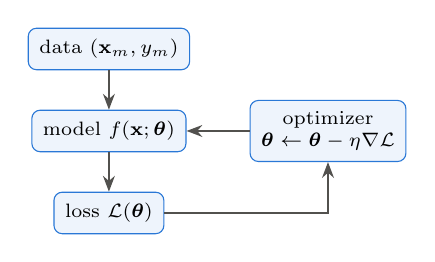
\begin{tikzpicture}[node distance=5mm]
        \node[box] (d) {data $(\bx_m, y_m)$};
        \node[box, below=of d] (m) {model $f(\bx;\btheta)$};
        \node[box, below=of m] (l) {loss $\mathcal L(\btheta)$};
        \node[box, right=8mm of m] (o) {optimizer\\$\btheta \leftarrow \btheta - \eta\nabla\mathcal L$};
        \draw[arr] (d) -- (m); \draw[arr] (m) -- (l); \draw[arr] (l) -| (o); \draw[arr] (o) -- (m);
      \end{tikzpicture}
      \begin{exampleblock}{In \texttt{QML.ipynb}}
        \scriptsize $\bx$ = 8 pixel values, $y = \pm1$ (horizontal / vertical line), $f$ = a quantum circuit, $\btheta$ = 12 angles.
      \end{exampleblock}
    \end{column}
  \end{columns}
\end{frame}

\begin{frame}[label=fKinds]{Kinds of learning; classification and regression}
  \begin{columns}[T]
    \begin{column}{0.5\textwidth}
      \small
      \begin{block}{Supervised learning}
        Labelled pairs $(\bx_m, y_m)$; learn $\bx \mapsto y$.
        \begin{itemize}\itemsep0pt
          \item \key{classification}: $y$ from a finite set (spam / not spam, horizontal / vertical)
          \item \key{regression}: $y \in \mathbb R$ (price, energy)
        \end{itemize}
      \end{block}
      \begin{block}{Unsupervised learning}
        Only $\bx_m$; find structure: \key{clustering} ($k$-means), \key{dimensionality reduction} (PCA), density estimation, generative models.
      \end{block}
    \end{column}
    \begin{column}{0.46\textwidth}
      \small
      \begin{block}{Reinforcement learning}
        An agent acts, receives rewards, and learns a policy that maximises the long-term reward.
      \end{block}
      \begin{exampleblock}{Outputs}
        \scriptsize
        Binary classifier: score $f \in \mathbb R$, prediction $\hat y = \operatorname{sign} f$ (labels $\pm1$) or probability $p = \sigma(f)$
        (labels $0/1$).\\
        Multi-class: softmax $p_k = e^{z_k}/\sum_je^{z_j}$.\\
        Regression: $\hat y = f$ directly.
      \end{exampleblock}
      \small QML has versions of all three; this repository implements \key{supervised binary classification}.
    \end{column}
  \end{columns}
\end{frame}

\begin{frame}[label=fSplit]{Training, validation and test data}
  \begin{columns}[T]
    \begin{column}{0.55\textwidth}
      \small
      \begin{itemize}\itemsep2pt
        \item \key{Training set}: fit the parameters $\btheta$.
        \item \key{Validation set}: choose hyper-parameters (learning rate, depth, \dots).
        \item \key{Test set}: estimate performance on new data --- used \emph{once}, at the end.
      \end{itemize}
      \begin{alertblock}{Data leakage}
        \scriptsize Fitting a scaler on all data, or picking hyper-parameters by test score, makes the reported accuracy
        optimistic. Split first; fit everything on the training split.
      \end{alertblock}
    \end{column}
    \begin{column}{0.41\textwidth}
      \begin{exampleblock}{\texttt{QML.ipynb} \tagimpl}
        \scriptsize
        \texttt{train\_x, train\_y = make\_images(20)}\\
        \texttt{test\_x, test\_y = make\_images(20)}\\[2pt]
        Two independent draws from the same generator (seed 42): 20 training and 20 test images, half
        horizontal, half vertical. No validation split: there is no hyper-parameter search.
      \end{exampleblock}
      \small A test set of 20 images gives an accuracy with a standard error of about $\pm\numsetwenty$ points
      (slide ``uncertainty'').
    \end{column}
  \end{columns}
\end{frame}

\begin{frame}[label=fFeat]{Feature engineering}
  \begin{columns}[T]
    \begin{column}{0.5\textwidth}
      \small
      Features are the numbers the model sees. Good features can make a hard task easy.
      \begin{itemize}\itemsep0pt
        \item \key{raw}: the 8 pixel brightnesses $x_i \in [0, 1]$
        \item \key{scaling}: a fixed range, needed for angle encoding ($x\mapsto\pi x$)
        \item \key{engineered}: brightest horizontal pair vs.\ brightest vertical pair
      \end{itemize}
    \end{column}
    \begin{column}{0.46\textwidth}
      \begin{exampleblock}{A hand-made rule \tagillus}
        \scriptsize ``Horizontal if some horizontal neighbour pair is brighter than every vertical pair.''
        No training: \numruletest\,\% test accuracy (\numbigrule\,\% on 2000 fresh images). Lesson: compare quantum models with simple
        classical methods \emph{on the same features}.
      \end{exampleblock}
    \end{column}
  \end{columns}
  \centering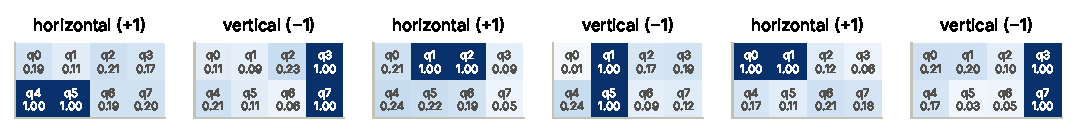
\includegraphics[width=0.9\textwidth]{dataset}\\[-2pt]
  {\scriptsize The first six training images of \texttt{QML.ipynb} with pixel values; pixel (row $r$, column $c$) becomes qubit $4r + c$.}
\end{frame}

\begin{frame}[label=fLoss]{Loss functions}
  \footnotesize
  \begin{center}
  \renewcommand{\arraystretch}{1.25}
\resizebox{\linewidth}{!}{%
  \begin{tabular}{llll}
    \toprule
    \textbf{Loss} & \textbf{Formula (one example)} & \textbf{Used for} & \textbf{Note}\\ \midrule
    mean squared error & $(f - y)^2$ & regression; \texttt{QML.ipynb} with $y = \pm1$ & punishes small margins\\
    binary cross-entropy & $-[y\ln p + (1 - y)\ln(1 - p)]$ & probabilities, $y \in \{0, 1\}$ & $\partial/\partial z = p - y$ for $p = \sigma(z)$\\
    cross-entropy & $-\ln p_{\text{true}}$, $p = \operatorname{softmax}(\mathbf z)$ & multi-class & \\
    hinge & $\max(0, 1 - yf)$ & SVM & zero once the margin is 1\\ \bottomrule
  \end{tabular}}
  \end{center}
  \begin{columns}[T]
    \begin{column}{0.5\textwidth}
      \begin{exampleblock}{Worked example: MSE vs.\ accuracy}
        \scriptsize Outputs $0.6, -0.2, 0.9, 0.1$, labels $+1, -1, +1, -1$:\\
        errors $-0.4, 0.8, -0.1, 1.1$; MSE $= \frac{0.16 + 0.64 + 0.01 + 1.21}{4} = 0.505$;\\
        signs correct for 3 of 4: accuracy $75\,\%$.
      \end{exampleblock}
    \end{column}
    \begin{column}{0.46\textwidth}
      \begin{block}{Training objective}
        \scriptsize $\displaystyle\mathcal L(\btheta) = \frac1M\sum_{m=1}^{M}\ell\big(f(\bx_m;\btheta), y_m\big)$, the average over the training set.
        The notebook uses $\ell = (f - y)^2$ with $f = \langle Z_{\text{out}}\rangle \in [-1, 1]$.
      \end{block}
    \end{column}
  \end{columns}
\end{frame}

\begin{frame}[label=fGD]{Gradient descent}
  \begin{columns}[T]
    \begin{column}{0.52\textwidth}
      \small
      The gradient $\nabla\mathcal L$ points uphill; step downhill:
      \[ \btheta \leftarrow \btheta - \eta\,\nabla\mathcal L(\btheta), \qquad \eta = \text{learning rate}. \]
      \begin{itemize}\itemsep1pt
        \item $\eta$ too small: slow; too large: divergence. For a quadratic with curvature $\lambda_{\max}$, stable iff $\eta < 2/\lambda_{\max}$.
        \item \key{stochastic} GD: gradient of a random mini-batch.
        \item \key{momentum}: $v \leftarrow \beta v + \nabla\mathcal L$, $\btheta \leftarrow \btheta - \eta v$; Adam adds per-parameter step sizes.
        \item \key{gradient-free} methods (COBYLA, Nelder--Mead) use only loss values.
      \end{itemize}
    \end{column}
    \begin{column}{0.44\textwidth}
      \begin{exampleblock}{Worked example}
        \scriptsize
        $\mathcal L = (w_1 - 3)^2 + 2(w_2 + 1)^2$,\\ start $(0, 0)$, $\eta = 0.1$.\\
        $\nabla\mathcal L = (2(w_1 - 3),\ 4(w_2 + 1)) = (-6, 4)$.\\
        New point $(0, 0) - 0.1(-6, 4) = (0.6, -0.4)$.\\
        Loss: $11 \to 5.76 + 0.72 = 6.48$.
      \end{exampleblock}
      \begin{alertblock}{In \texttt{QML.ipynb}}
        \scriptsize COBYLA (gradient-free, \tagimpl) with 100 loss evaluations; no gradients are computed.
      \end{alertblock}
    \end{column}
  \end{columns}
\end{frame}

\begin{frame}[label=fNN]{Neural networks}
  \begin{columns}[T]
    \begin{column}{0.5\textwidth}
      \small
      A \key{neuron}: $a = \phi(\mathbf w\cdot\bx + b)$ with an activation $\phi$.\\
      A \key{layer}: $\mathbf h = \phi(W\bx + \mathbf b)$; layers are stacked.
      \begin{itemize}\itemsep1pt
        \item activations: sigmoid $\sigma$, $\tanh$, ReLU $\max(0, z)$
        \item derivatives: $\sigma' = \sigma(1 - \sigma)$, $\tanh' = 1 - \tanh^2$, ReLU$' = [z > 0]$
        \item without non-linear activations the network is linear and cannot solve XOR
        \item \key{CNNs} share the weights of small filters over the image and pool to reduce size --- the template for the QCNN
      \end{itemize}
    \end{column}
    \begin{column}{0.46\textwidth}
      \centering
      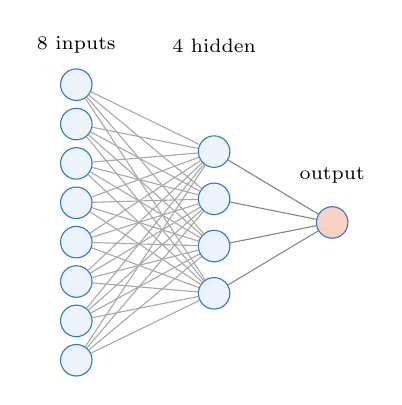
\begin{tikzpicture}[x=1.25cm, y=0.5cm, n/.style={circle, draw=qblue, fill=qlight, minimum size=4mm, inner sep=0}]
        \foreach \i in {1,...,8} \node[n] (i\i) at (0, -\i) {};
        \foreach \j in {1,...,4} \node[n] (h\j) at (1.4, -1.2*\j - 1.5) {};
        \node[n, fill=qorange!30] (o) at (2.6, -4.5) {};
        \foreach \i in {1,...,8} \foreach \j in {1,...,4} \draw[qgrey!50] (i\i) -- (h\j);
        \foreach \j in {1,...,4} \draw[qgrey!70] (h\j) -- (o);
        \node[font=\scriptsize] at (0, 0) {8 inputs}; \node[font=\scriptsize] at (1.4, 0) {4 hidden}; \node[font=\scriptsize] at (2.6, -3.3) {output};
      \end{tikzpicture}\\
      {\scriptsize $8\cdot4 + 4 + 4\cdot1 + 1 = 41$ parameters. The 8-qubit QCNN has \numnparams.}
    \end{column}
  \end{columns}
\end{frame}

\begin{frame}[label=fBackprop]{Back-propagation: the chain rule, worked}
  \begin{columns}[T]
    \begin{column}{0.5\textwidth}
      \small
      Network: $\mathbf h = \operatorname{ReLU}(W_1\bx + \mathbf b_1)$, $p = \sigma(\mathbf w_2\cdot\mathbf h + b_2)$, loss $L = -\ln p$ ($y = 1$).
      \[ W_1 = \begin{pmatrix}1 & -1\\ 2 & 1\end{pmatrix},\quad \mathbf b_1 = (0, -2), \]\[ \mathbf w_2 = (0.5, -1),\quad b_2 = -1. \]
      \key{Forward}, $\bx = (1, -1)$: $\mathbf a = (2, -1)$, $\mathbf h = (2, 0)$, $z = 0$, $p = \frac12$, $L = \ln2$.
    \end{column}
    \begin{column}{0.46\textwidth}
      \small
      \key{Backward}:
      \begin{itemize}\itemsep1pt
        \item $\partial L/\partial z = p - y = -0.5$ (sigmoid + cross-entropy)
        \item $\partial L/\partial\mathbf w_2 = -0.5\,\mathbf h = (-1, 0)$, $\partial L/\partial b_2 = -0.5$
        \item $\partial L/\partial a_j = -0.5\,w_{2,j}[a_j > 0] = (-0.25, 0)$
        \item $\partial L/\partial W_1 = \begin{pmatrix}-0.25 & 0.25\\ 0 & 0\end{pmatrix}$: the inactive ReLU gets no gradient
      \end{itemize}
      \begin{block}{Quantum analogue}
        \scriptsize A quantum circuit cannot be back-propagated through on hardware; its derivatives come from extra circuit runs
        (parameter shift, Part C).
      \end{block}
    \end{column}
  \end{columns}
\end{frame}

\begin{frame}[label=fFit]{Overfitting and underfitting}
  \begin{columns}[T]
    \begin{column}{0.52\textwidth}
      \small
      \begin{itemize}\itemsep2pt
        \item \key{Underfitting} (high bias): training and test errors both high. Remedy: more capacity, better features.
        \item \key{Overfitting} (high variance): training error low, test error high. Remedy: regularisation
          ($+\lambda\|\btheta\|^2$), more data, simpler model, early stopping.
        \item The \key{generalisation gap} is test error minus training error.
        \item Regularisation \emph{raises} the training error on purpose to lower the test error.
      \end{itemize}
    \end{column}
    \begin{column}{0.44\textwidth}
      \centering
      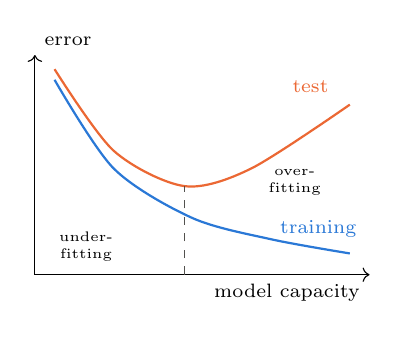
\begin{tikzpicture}[x=0.5cm, y=0.45cm]
        \draw[->] (0,0) -- (8.5,0) node[below left, font=\scriptsize]{model capacity};
        \draw[->] (0,0) -- (0,6.2) node[above right, font=\scriptsize]{error};
        \draw[qblue, thick] plot[smooth] coordinates {(0.5,5.5) (2,3) (4,1.6) (6,1) (8,0.6)};
        \draw[qorange, thick] plot[smooth] coordinates {(0.5,5.8) (2,3.5) (3.8,2.5) (5.5,3) (8,4.8)};
        \node[qblue, font=\scriptsize] at (7.2,1.3) {training};
        \node[qorange, font=\scriptsize] at (7.0,5.3) {test};
        \draw[dashed, qgrey] (3.8,0) -- (3.8,2.5);
        \node[font=\tiny, align=center] at (1.3,0.8) {under-\\fitting}; \node[font=\tiny, align=center] at (6.6,2.6) {over-\\fitting};
      \end{tikzpicture}
      \begin{exampleblock}{Recorded QCNN run}
        \scriptsize training accuracy \numtrainacc\,\%, test accuracy \numtestacc\,\%: a small gap --- with only 12 parameters there is little room to overfit.
      \end{exampleblock}
    \end{column}
  \end{columns}
\end{frame}

\begin{frame}[label=fEval]{Model evaluation: confusion matrix and metrics}
  \begin{columns}[T]
    \begin{column}{0.5\textwidth}
      \small
      Positive class = ``horizontal''.
      \begin{center}\footnotesize
      \begin{tabular}{lcc}\toprule & pred.\ H & pred.\ V\\ \midrule
      true H & TP & FN\\ true V & FP & TN\\ \bottomrule\end{tabular}
      \end{center}
      \begin{itemize}\itemsep0pt\footnotesize
        \item accuracy $= \frac{TP + TN}{\text{all}}$
        \item precision $= \frac{TP}{TP + FP}$ (how many alarms are right)
        \item recall $= \frac{TP}{TP + FN}$ (how many positives are found)
        \item $F_1 = \frac{2PR}{P + R} = \frac{2TP}{2TP + FP + FN}$
        \item loss (MSE) measures confidence, not only correctness
      \end{itemize}
    \end{column}
    \begin{column}{0.46\textwidth}
      \begin{exampleblock}{QCNN test set (re-executed run)}
        \footnotesize
        \begin{center}
        \begin{tabular}{lcc}\toprule & pred.\ H & pred.\ V\\ \midrule
        true H & \numtesttp & \numtestfn\\ true V & \numtestfp & \numtesttn\\ \bottomrule\end{tabular}
        \end{center}
        accuracy $= \numtestacc\,\%$, precision $= \numtestprec$, recall $= \numtestrec$, $F_1 = \numtestfone$, test MSE $= \numtestloss$.
      \end{exampleblock}
      \scriptsize The notebook prints accuracy and loss only; precision, recall and F1 were computed for this lecture from the same outputs.
    \end{column}
  \end{columns}
\end{frame}

\begin{frame}[label=fUnc]{How certain is an accuracy?}
  \begin{columns}[T]
    \begin{column}{0.52\textwidth}
      \small
      The number of correct test predictions is binomial. The estimated accuracy $\hat a$ on $M$ images has
      \[ \mathrm{SE}(\hat a) = \sqrt{\frac{\hat a(1 - \hat a)}{M}}. \]
      \begin{itemize}\itemsep1pt
        \item $M = 20$, $\hat a = 0.85$: $\mathrm{SE} = 0.080$ --- the 95\,\% range is roughly $69$--$100\,\%$.
        \item $M = 2000$: $\mathrm{SE} \approx 0.009$.
      \end{itemize}
      \begin{exampleblock}{Measured \tagillus}
        \scriptsize The trained QCNN on 2000 fresh images from the same generator: \numbigacc\,\% --- consistent with $85 \pm 8\,\%$ on 20 images.
      \end{exampleblock}
    \end{column}
    \begin{column}{0.44\textwidth}
      \begin{alertblock}{Rules of thumb}
        \small
        \begin{itemize}\itemsep1pt
          \item report the test-set size and an error bar
          \item never compare models on a few dozen images
          \item fix the seed for reproducibility, but test several seeds for robustness
        \end{itemize}
      \end{alertblock}
    \end{column}
  \end{columns}
\end{frame}

\begin{frame}[label=fCvQ]{Classical ML versus quantum ML}
  \scriptsize
  \begin{center}
  \renewcommand{\arraystretch}{1.12}
  \resizebox{\linewidth}{!}{%
\begin{tabular}{p{3.0cm}p{5.2cm}p{5.2cm}}
    \toprule & \textbf{Classical ML} & \textbf{(Hybrid) quantum ML}\\ \midrule
    model & neural network, kernel machine, tree, \dots & parameterized quantum circuit + classical optimizer\\
    data in the model & numbers in memory & encoded into a quantum state (costs gates)\\
    output & any real number, read directly & expectation values, estimated from \emph{shots}\\
    gradients & back-propagation (one backward pass) & extra circuit runs per parameter (parameter shift)\\
    state space & $d$ numbers & $2^n$ amplitudes, not directly readable\\
    maturity & huge models, GPUs, mature tools & small, noisy devices; mostly simulated today\\
    advantage & --- & \hl{not demonstrated} for practical classical data\\ \bottomrule
  \end{tabular}}
  \end{center}
  \small Hybrid = a quantum circuit inside a classical training loop. This is what \texttt{QML.ipynb} implements.
\end{frame}

% =====================================================================================
\section{Part B: Quantum computing foundations}
\begin{frame}[label=fQubit]{Qubits, superposition and measurement}
  \begin{columns}[T]
    \begin{column}{0.52\textwidth}
      \small
      A qubit state is a unit vector
      \[ \ket\psi = \alpha\ket0 + \beta\ket1 = \begin{pmatrix}\alpha\\ \beta\end{pmatrix},\quad |\alpha|^2 + |\beta|^2 = 1, \]
      $\alpha, \beta \in \mathbb C$ are \key{amplitudes}. \key{Superposition}: both are non-zero.\\[3pt]
      \key{Born rule}: measuring gives $0$ with probability $|\alpha|^2$, $1$ with probability $|\beta|^2$; the state collapses.
      \begin{itemize}\itemsep0pt
        \item global phase $e^{i\phi}\ket\psi$: unobservable
        \item relative phase ($\ket+$ vs.\ $\ket-$): observable after a change of basis
      \end{itemize}
    \end{column}
    \begin{column}{0.44\textwidth}
      \begin{exampleblock}{Worked example}
        \scriptsize $\ket\psi = \frac12\ket0 + \frac{\sqrt3}{2}e^{i\pi/4}\ket1$:\\
        $P(0) = \frac14$, $P(1) = \frac34$,\\
        $\langle Z\rangle = P(0) - P(1) = -\frac12$,\\
        $\langle X\rangle = 2\operatorname{Re}(\alpha^*\beta) = \frac{\sqrt3}{2}\cos\frac\pi4 = \frac{\sqrt6}{4}$.
      \end{exampleblock}
      \begin{block}{Shots}
        \scriptsize Each run gives one bit. With $S$ shots, $\widehat{\langle Z\rangle}$ has error $\sqrt{(1 - \langle Z\rangle^2)/S} \approx 1/\sqrt S$.
        1000 shots, 620 zeros: $\langle Z\rangle \approx 0.24 \pm 0.03$.
      \end{block}
    \end{column}
  \end{columns}
\end{frame}

\begin{frame}[label=fBloch]{The Bloch sphere}
  \begin{columns}[T]
    \begin{column}{0.44\textwidth}
      \centering
      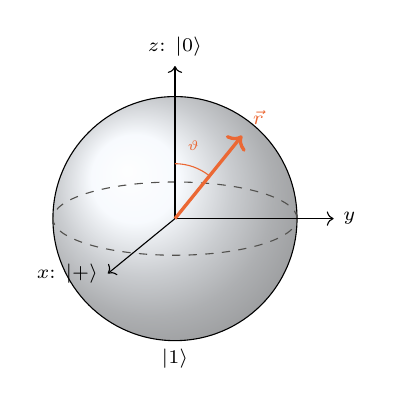
\begin{tikzpicture}[scale=1.55]
        \shade[ball color=qlight, opacity=0.6] (0,0) circle (1);
        \draw (0,0) circle (1);
        \draw[dashed, qgrey] (0,0) ellipse (1 and 0.3);
        \draw[->] (0,0) -- (0,1.25) node[above, font=\scriptsize]{$z$: $\ket0$};
        \draw[->] (0,0) -- (-0.55,-0.45) node[left, font=\scriptsize]{$x$: $\ket+$};
        \draw[->] (0,0) -- (1.3,0) node[right, font=\scriptsize]{$y$};
        \node[font=\scriptsize] at (0,-1.15) {$\ket1$};
        \draw[->, very thick, qorange] (0,0) -- (0.55,0.68) node[above right, font=\scriptsize]{$\vec r$};
        \draw[qorange] (0,0.45) arc (90:51:0.45); \node[font=\tiny, qorange] at (0.15,0.6) {$\vartheta$};
      \end{tikzpicture}
    \end{column}
    \begin{column}{0.52\textwidth}
      \small
      Every pure state can be written
      \[ \ket\psi = \cos\tfrac\vartheta2\ket0 + e^{i\varphi}\sin\tfrac\vartheta2\ket1 \]
      and drawn as the unit vector
      \[ \vec r = (\langle X\rangle, \langle Y\rangle, \langle Z\rangle) \]\[ = (\sin\vartheta\cos\varphi,\ \sin\vartheta\sin\varphi,\ \cos\vartheta). \]
      \begin{itemize}\itemsep0pt
        \item gates = rotations of the sphere; $R_Y(\theta)$ turns $\vec r$ about the $y$-axis
        \item note the \hl{half angle}: $\vartheta = \frac\pi4$ means amplitudes $\cos\frac\pi8, \sin\frac\pi8$
        \item notebook encoding $R_Y(\pi x)\ket0$: pixel $x$ $\mapsto$ polar angle $\pi x$; dark at the north pole, lit at the south pole
      \end{itemize}
    \end{column}
  \end{columns}
\end{frame}

\begin{frame}[label=fTensor]{Tensor products: many qubits}
  \begin{columns}[T]
    \begin{column}{0.52\textwidth}
      \small
      $n$ qubits live in $\mathbb C^{2^n}$; basis states $\ket{q_0q_1\dots q_{n-1}}$ (qubit 0 written first, as CUDA-Q prints them).
      \[ \ket a\otimes\ket b = \begin{pmatrix}a_0b_0\\ a_0b_1\\ a_1b_0\\ a_1b_1\end{pmatrix},\quad
         A\otimes B = \begin{pmatrix}a_{11}B & a_{12}B\\ a_{21}B & a_{22}B\end{pmatrix}. \]
      \begin{exampleblock}{Worked example}
        \scriptsize $R_Y(\frac\pi2)\ket0\otimes R_Y(\pi)\ket0 = \frac{1}{\sqrt2}(\ket0 + \ket1)\otimes\ket1 = \frac{1}{\sqrt2}(0, 1, 0, 1)^{\mathsf T}$.
      \end{exampleblock}
    \end{column}
    \begin{column}{0.44\textwidth}
      \begin{alertblock}{Exponential memory}
        \small A state vector stores $2^n$ complex numbers: $16\cdot2^n$ bytes in double precision.
        \begin{center}\footnotesize
        \begin{tabular}{rr}\toprule $n$ & memory\\ \midrule 8 & 4 KB (notebook default)\\ 15 & 0.5 MB\\ 30 & 16 GiB\\ 32 & 64 GiB (one 80 GB GPU)\\ 34 & 256 GiB (four GPUs)\\ \bottomrule\end{tabular}
        \end{center}
      \end{alertblock}
    \end{column}
  \end{columns}
\end{frame}

\begin{frame}[label=fEnt]{Entanglement}
  \begin{columns}[T]
    \begin{column}{0.5\textwidth}
      \small
      A two-qubit pure state $\sum c_{ab}\ket{ab}$ is a \key{product state} iff $c_{00}c_{11} - c_{01}c_{10} = 0$; otherwise it is \key{entangled}.
      \begin{center}
      \begin{quantikz}[row sep=0.3cm, column sep=0.45cm]
        \lstick{$\ket0$} & \gate{H} & \ctrl{1} & \qw \\
        \lstick{$\ket0$} & \qw & \targ{} & \qw
      \end{quantikz}
      \end{center}
      $\ket{\Phi^+} = \frac{1}{\sqrt2}(\ket{00} + \ket{11})$: $\langle Z_0\rangle = \langle Z_1\rangle = 0$, but $\langle Z_0Z_1\rangle = \langle X_0X_1\rangle = 1$.
    \end{column}
    \begin{column}{0.46\textwidth}
      \begin{exampleblock}{Entanglement hides local information}
        \scriptsize Apply $R_Y(\theta)$ to qubit 1 of $\ket{\Phi^+}$: its reduced state is $\frac I2$, so $\langle Z_1\rangle = 0$ for \emph{every} $\theta$,
        while $\langle Z_0Z_1\rangle = \cos\theta$.\\[2pt]
        A one-qubit readout can be blind to a parameter --- a first glimpse of barren plateaus.
      \end{exampleblock}
      \begin{block}{Measuring entanglement}
        \scriptsize Purity of the reduced state $\operatorname{tr}\rho_1^2 \in [\frac12, 1]$: $1$ = product, $\frac12$ = maximally entangled.
        For $\cos\frac\theta2\ket{00} + \sin\frac\theta2\ket{11}$: $\operatorname{tr}\rho_1^2 = \frac{1 + \cos^2\theta}{2}$.
      \end{block}
    \end{column}
  \end{columns}
\end{frame}

\begin{frame}[label=fGates]{Quantum gates are unitary matrices}
  \begin{columns}[T]
    \begin{column}{0.55\textwidth}
      \footnotesize
\resizebox{\linewidth}{!}{%
      \begin{tabular}{lll}
        \toprule gate & matrix & action\\ \midrule
        $X, Y, Z$ & Pauli matrices & bit flip, both, phase flip\\
        $H$ & $\frac{1}{\sqrt2}\begin{psmallmatrix}1&1\\1&-1\end{psmallmatrix}$ & $\ket0 \to \ket+$; $HZH = X$\\
        $S$ & $\operatorname{diag}(1, i)$ & $SXS^\dagger = Y$\\
        $R_P(\theta)$ & $e^{-i\theta P/2} = \cos\frac\theta2I - i\sin\frac\theta2P$ & rotation by $\theta$ about axis $P$\\
        CNOT & $\ket0\!\bra0\otimes I + \ket1\!\bra1\otimes X$ & flips the target if control $= 1$\\
        C-$U$ & $\ket0\!\bra0\otimes I + \ket1\!\bra1\otimes U$ & e.g.\ \texttt{rz.ctrl}, \texttt{rx.ctrl}\\ \bottomrule
      \end{tabular}}\\[4pt]
      Pauli algebra: $X^2 = Y^2 = Z^2 = I$, $XY = iZ = -YX$ (cyclic); so $(aX + bY + cZ)^2 = (a^2 + b^2 + c^2)I$.
    \end{column}
    \begin{column}{0.41\textwidth}
      \begin{block}{Unitary: $U^\dagger U = I$}
        \scriptsize Columns orthonormal; reversible; preserves the norm. $\frac{1}{\sqrt2}\begin{psmallmatrix}1&1\\1&1\end{psmallmatrix}$ is \emph{not} unitary.
      \end{block}
      \begin{exampleblock}{Controlled-$R_Z$, basis $\ket{00},\ket{01},\ket{10},\ket{11}$}
        \scriptsize $\operatorname{diag}(1, 1, e^{-i\theta/2}, e^{i\theta/2})$ --- not the controlled-phase $\operatorname{diag}(1,1,1,e^{i\theta})$:
        they differ by a relative phase.
      \end{exampleblock}
      \begin{block}{Heisenberg picture}
        \scriptsize $R_Y(\theta)^\dagger ZR_Y(\theta) = \cos\theta\,Z - \sin\theta\,X$.
      \end{block}
    \end{column}
  \end{columns}
\end{frame}

\begin{frame}[label=fCirc]{Quantum circuits and expectation values}
  \begin{columns}[T]
    \begin{column}{0.5\textwidth}
      \small
      Read circuits left to right; each wire is a qubit; boxes are gates; the meter is a measurement.
      \begin{center}
      \begin{quantikz}[row sep=0.3cm, column sep=0.4cm]
        \lstick{$q_0:\ \ket0$} & \gate{R_Y(\theta)} & \ctrl{1} & \meter{} \\
        \lstick{$q_1:\ \ket0$} & \qw & \targ{} & \meter{}
      \end{quantikz}
      \end{center}
      \scriptsize State: $\cos\frac\theta2\ket{00} + \sin\frac\theta2\ket{11}$; $\langle Z_1\rangle = \cos\theta$, $\langle Z_0Z_1\rangle = 1$.
    \end{column}
    \begin{column}{0.46\textwidth}
      \small
      \key{Expectation value} of an observable $M$ (Hermitian):
      \[ \langle M\rangle = \braket{\psi|M|\psi} = \sum_k\lambda_kP(\lambda_k). \]
      In CUDA-Q:
      \begin{itemize}\itemsep0pt\scriptsize
        \item \texttt{cudaq.sample(kernel)}: bitstring counts (qubit 0 first)
        \item \texttt{cudaq.observe(kernel, cudaq.spin.z(7), ...)}: $\langle Z_7\rangle$, \emph{exact} on a state-vector simulator, estimated with \texttt{shots\_count}
      \end{itemize}
      \begin{exampleblock}{From counts}
        \scriptsize \texttt{\{00:400, 01:100, 10:300, 11:200\}}: $\langle Z_0\rangle = 0$, $\langle Z_1\rangle = 0.4$, $\langle Z_0Z_1\rangle = 0.2$.
      \end{exampleblock}
    \end{column}
  \end{columns}
\end{frame}

\begin{frame}[label=fPQC]{Parameterized quantum circuits}
  \begin{columns}[T]
    \begin{column}{0.52\textwidth}
      \small
      A \key{parameterized quantum circuit} (PQC) $U(\btheta)$ contains gates whose angles are trainable numbers. Its model output is
      \[ f(\btheta) = \braket{0|U(\btheta)^\dagger\,M\,U(\btheta)|0}. \]
      \key{Key fact}: if $\theta_k$ appears in \emph{one} gate $e^{-i\theta_kP/2}$, then
      \[ f = a + b\cos\theta_k + c\sin\theta_k \]
      (period $2\pi$, three numbers determine it).
    \end{column}
    \begin{column}{0.44\textwidth}
      \begin{exampleblock}{Worked example}
        \scriptsize $R_X(\theta_2)R_Y(\theta_1)\ket0$: Bloch vector $(0,0,1) \xrightarrow{R_Y} (\sin\theta_1, 0, \cos\theta_1) \xrightarrow{R_X}$\\
        $z = \cos\theta_1\cos\theta_2$. So $f(\theta_1, \theta_2) = \cos\theta_1\cos\theta_2$ --- trigonometric in each angle separately,
        not $\cos(\theta_1 + \theta_2)$.
      \end{exampleblock}
      \begin{block}{Why trigonometric?}
        \scriptsize $e^{-i\theta P/2}$ has eigenvalues $e^{\mp i\theta/2}$; $f$ multiplies the ket and bra factors, giving frequencies $0$ and $1$ in $\theta$.
      \end{block}
    \end{column}
  \end{columns}
\end{frame}

\begin{frame}[label=fPrep]{Quantum state preparation}
  \begin{columns}[T]
    \begin{column}{0.52\textwidth}
      \small
      Every QML model starts by \key{preparing a state} from classical numbers.
      \begin{itemize}\itemsep1pt
        \item a product of single-qubit rotations: $n$ gates, depth 1 (angle encoding)
        \item a basis state $\ket{b}$: at most $n$ $X$ gates
        \item an arbitrary state of $n$ qubits: in general $\Theta(2^n)$ gates (Möttönen-type or Shende--Bullock--Markov constructions)
        \item simulators can load a vector directly: \texttt{cudaq.qvector(vector)} \tagimpl{} in \texttt{HHL.ipynb}, \texttt{QFT.ipynb} --- not available on hardware in this form
      \end{itemize}
    \end{column}
    \begin{column}{0.44\textwidth}
      \begin{alertblock}{The data-loading bottleneck}
        \small If loading $N$ numbers costs $O(N)$ gates, any algorithm that then runs in $O(\log N)$ is dominated by loading.
        Claims of exponential QML speed-ups usually \emph{assume} a cheap loader (e.g.\ QRAM), which does not exist at scale today.
      \end{alertblock}
    \end{column}
  \end{columns}
\end{frame}

% =====================================================================================
\section{Part C: QML fundamentals}
\begin{frame}[label=fQML]{What is quantum machine learning? Quantum and classical data}
  \begin{columns}[T]
    \begin{column}{0.48\textwidth}
      \centering
      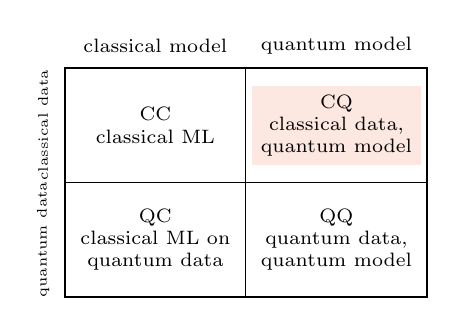
\begin{tikzpicture}[x=2.3cm, y=1.45cm]
        \draw[thick] (0,0) rectangle (2,2); \draw (1,0) -- (1,2); \draw (0,1) -- (2,1);
        \node[font=\scriptsize, align=center] at (0.5,1.5) {CC\\classical ML};
        \node[font=\scriptsize, align=center, fill=qorange!15] at (1.5,1.5) {CQ\\classical data,\\quantum model};
        \node[font=\scriptsize, align=center] at (0.5,0.5) {QC\\classical ML on\\quantum data};
        \node[font=\scriptsize, align=center] at (1.5,0.5) {QQ\\quantum data,\\quantum model};
        \node[font=\scriptsize] at (0.5,2.2) {classical model}; \node[font=\scriptsize] at (1.5,2.2) {quantum model};
        \node[font=\tiny, rotate=90] at (-0.12,1.5) {classical data}; \node[font=\tiny, rotate=90] at (-0.12,0.5) {quantum data};
      \end{tikzpicture}\\
      {\scriptsize \texttt{QML.ipynb} is in the CQ corner.}
    \end{column}
    \begin{column}{0.48\textwidth}
      \small
      \begin{itemize}\itemsep2pt
        \item \key{Classical data}: images, tables, text --- must be \emph{encoded} into qubits (costly, Part C).
        \item \key{Quantum data}: states produced by a quantum process (a sensor, a simulation, a phase of matter) --- already
          quantum; this is where the strongest theoretical advantages are known.
        \item \key{Hybrid QML}: a quantum circuit computes features or outputs; a classical computer computes the loss and updates the parameters.
      \end{itemize}
    \end{column}
  \end{columns}
\end{frame}

\begin{frame}[label=fEnc]{Classical-to-quantum data encoding}
  \footnotesize
  \begin{center}
  \renewcommand{\arraystretch}{1.3}
\resizebox{\linewidth}{!}{%
  \begin{tabular}{lllll}
    \toprule \textbf{Encoding} & \textbf{State} & \textbf{Qubits} & \textbf{Gates} & \textbf{Notes}\\ \midrule
    basis & $\ket{b_1b_2\dots b_n}$ & 1 per bit & $\le n$ $X$ & binary data only\\
    angle & $\bigotimes_iR_Y(x_i)\ket0$ & 1 per feature & $d$, depth 1 & product state; \texttt{QML.ipynb} uses $R_Y(\pi x_i)$\\
    amplitude & $\frac{1}{\|\bx\|}\sum_jx_j\ket j$ & $\lceil\log_2d\rceil$ & $O(d)$ in general & exponentially compact\\
    feature map & $U_\Phi(\bx)\ket{0}^{\otimes n}$ & 1 per feature & problem dependent & entangling (e.g.\ ZZ map)\\
    re-uploading & $\prod_l W_l\,S(\bx)$ & any & $L$ copies of $S(\bx)$ & richer functions of $\bx$\\ \bottomrule
  \end{tabular}}
  \end{center}
  \begin{exampleblock}{Resource example}
    \scriptsize $d = 256$ features of 8 bits each: basis encoding $2048$ qubits, angle encoding $256$ qubits, amplitude encoding $8$ qubits.
    Fewer qubits $\Rightarrow$ deeper state preparation.
  \end{exampleblock}
\end{frame}

\begin{frame}[label=fBasisAmp]{Basis and amplitude encoding: worked examples}
  \begin{columns}[T]
    \begin{column}{0.46\textwidth}
      \begin{block}{Basis encoding}
        \small $5 = 101_2 \mapsto \ket{101}$: apply $X$ to qubits 0 and 2.
        \begin{center}
        \begin{quantikz}[row sep=0.2cm, column sep=0.4cm]
          \lstick{$\ket0$} & \gate{X} & \qw \\
          \lstick{$\ket0$} & \qw & \qw \\
          \lstick{$\ket0$} & \gate{X} & \qw
        \end{quantikz}
        \end{center}
        \scriptsize A superposition of many data strings can be prepared, but reading out results needs many measurements.
      \end{block}
    \end{column}
    \begin{column}{0.5\textwidth}
      \begin{exampleblock}{Amplitude encoding}
        \small $\bx = (1, 2, 4, 2)$, $\|\bx\| = 5$:
        \[ \ket{\psi_{\bx}} = 0.2\ket{00} + 0.4\ket{01} + 0.8\ket{10} + 0.4\ket{11}. \]
        2 qubits for 4 numbers. $P(q_0 = 1) = 0.8^2 + 0.4^2 = 0.80$; $P(q_1 = 1) = 0.32$.\\[2pt]
        \scriptsize Only $|x_j|^2/\|\bx\|^2$ can be sampled; the norm is lost and must be stored classically.
      \end{exampleblock}
    \end{column}
  \end{columns}
\end{frame}

\begin{frame}[fragile,label=fAngle]{Angle encoding --- the encoding of \texttt{QML.ipynb} \tagimpl}
  \begin{columns}[T]
    \begin{column}{0.5\textwidth}
      \small
      Pixel $x_i \in [0, 1]$ $\to$ qubit $i$:
      \[ R_Y(\pi x_i)\ket0 = \cos\tfrac{\pi x_i}2\ket0 + \sin\tfrac{\pi x_i}2\ket1, \]
      \[ \ket{\psi(\bx)} = \bigotimes_{i=0}^{7}R_Y(\pi x_i)\ket0. \]
      \begin{itemize}\itemsep0pt
        \item dark $x = 0 \to \ket0$, lit $x = 1 \to \ket1$
        \item $\langle Z_i\rangle = \cos(\pi x_i)$
        \item 8 gates, depth 1, no entanglement yet
      \end{itemize}
    \end{column}
    \begin{column}{0.46\textwidth}
      \begin{exampleblock}{Worked example}
        \scriptsize $x = \frac13$: half-angle $\frac\pi6$; $P(1) = \sin^2\frac\pi6 = \frac14$, $\langle Z\rangle = \frac12$.\\
        $x = \frac14$: $\cos\frac\pi8\ket0 + \sin\frac\pi8\ket1$, Bloch vector $(\frac{1}{\sqrt2}, 0, \frac{1}{\sqrt2})$.
      \end{exampleblock}
\begin{lstlisting}
for i in range(len(pixels)):
    ry(np.pi * pixels[i], qubits[i])
\end{lstlisting}
      \scriptsize Row-by-row flattening: pixel $(r, c)$ of the $2\times4$ image is qubit $4r + c$.
    \end{column}
  \end{columns}
\end{frame}

\begin{frame}[label=fFMap]{Quantum feature maps}
  \begin{columns}[T]
    \begin{column}{0.52\textwidth}
      \small
      A \key{feature map} $\bx \mapsto \rho(\bx) = \ket{\psi(\bx)}\!\bra{\psi(\bx)}$ sends data into a $2^n$-dimensional space of states.
      Linear models in that space = non-linear models in $\bx$ (as with the XOR problem).\\[3pt]
      \key{ZZ feature map} (Havlíček et al.\ 2019) \tagtheory:
      \[ U_\Phi(\bx) = \exp\Big(i\sum_i\phi_i(\bx)Z_i + i\sum_{i<j}\phi_{ij}(\bx)Z_iZ_j\Big)H^{\otimes n}, \]
      applied twice, e.g.\ $\phi_i = x_i$, $\phi_{ij} = (\pi - x_i)(\pi - x_j)$.
    \end{column}
    \begin{column}{0.44\textwidth}
      \begin{center}
      \resizebox{\linewidth}{!}{%
      \begin{quantikz}[row sep=0.25cm, column sep=0.3cm]
        \lstick{$\ket0$} & \gate{H} & \gate{R_Z(\phi_0)} & \ctrl{1} & \qw & \ctrl{1} & \qw \\
        \lstick{$\ket0$} & \gate{H} & \gate{R_Z(\phi_1)} & \targ{} & \gate{R_Z(\phi_{01})} & \targ{} & \qw
      \end{quantikz}}
      \end{center}
      \scriptsize (one repetition, two qubits; $ZZ$ phase via CNOT--$R_Z$--CNOT; angle conventions differ by factors of 2)
      \begin{block}{Product vs.\ entangling maps}
        \scriptsize Angle encoding is a product map: its kernel factorises and is classically trivial. Entangling maps can produce kernels
        that are believed hard to compute classically --- which still does not guarantee that they are \emph{useful}.
      \end{block}
    \end{column}
  \end{columns}
\end{frame}

\begin{frame}[label=fKern]{Quantum kernels}
  \begin{columns}[T]
    \begin{column}{0.5\textwidth}
      \small
      Fidelity (quantum) kernel:
      \[ k(\bx, \bx') = |\braket{\psi(\bx)|\psi(\bx')}|^2 = \operatorname{tr}\big[\rho(\bx)\rho(\bx')\big]. \]
      Always symmetric and positive semi-definite (exactly; shot-noise estimates may not be).
      \begin{exampleblock}{Notebook encoding}
        \scriptsize $k(\bx, \bx') = \prod_i\cos^2\frac{\pi(x_i - x'_i)}2$; e.g.\ $\bx = (1, 0.5)$, $\bx' = (0.5, 0)$: $k = \frac12\cdot\frac12 = \frac14$.
        A closed classical formula!
      \end{exampleblock}
    \end{column}
    \begin{column}{0.46\textwidth}
      \small Estimating $k$ on a quantum computer:
      \begin{itemize}\itemsep0pt\scriptsize
        \item \key{compute--uncompute}: run $U(\bx')^\dagger U(\bx)$; $k = P(0\dots0)$
        \item \key{swap test}: $P(\text{ancilla} = 0) = \frac12(1 + k)$
      \end{itemize}
      \begin{center}
      \begin{quantikz}[row sep=0.2cm, column sep=0.35cm]
        \lstick{$\ket0$} & \gate{H} & \ctrl{2} & \gate{H} & \meter{} \\
        \lstick{$\ket\psi$} & \qw & \swap{1} & \qw & \qw \\
        \lstick{$\ket\phi$} & \qw & \targX{} & \qw & \qw
      \end{quantikz}
      \end{center}
      \scriptsize $M$ training points need $\binom M2$ kernel circuits ($190$ for $M = 20$).
    \end{column}
  \end{columns}
\end{frame}

\begin{frame}[label=fAnsatz]{Variational quantum circuits (ansatz)}
  \begin{columns}[T]
    \begin{column}{0.5\textwidth}
      \small
      A \key{variational circuit} (ansatz) $U(\btheta)$: layers of trainable rotations and fixed entangling gates.
      \begin{itemize}\itemsep1pt
        \item \key{hardware-efficient ansatz} (HEA): $R_Y, R_Z$ on every qubit + a CNOT/CZ ladder, repeated $L$ times --- used in \texttt{VQE.ipynb} \tagimpl
        \item \key{problem-inspired} ans\"atze: UCC (chemistry), QAOA (optimization), QCNN (translation-invariant data)
        \item more layers $\Rightarrow$ more expressive, but harder to train and noisier
      \end{itemize}
    \end{column}
    \begin{column}{0.46\textwidth}
      \begin{center}
      \begin{quantikz}[row sep=0.2cm, column sep=0.25cm]
        \lstick{$q_0$} & \gate{R_Y} & \gate{R_Z} & \ctrl{1} & \qw & \qw & \qw \\
        \lstick{$q_1$} & \gate{R_Y} & \gate{R_Z} & \control{} & \ctrl{1} & \qw & \qw \\
        \lstick{$q_2$} & \gate{R_Y} & \gate{R_Z} & \qw & \control{} & \ctrl{1} & \qw \\
        \lstick{$q_3$} & \gate{R_Y} & \gate{R_Z} & \qw & \qw & \control{} & \qw
      \end{quantikz}
      \end{center}
      \scriptsize One HEA layer ($2n$ parameters) as used in the barren-plateau experiment of Part E.
    \end{column}
  \end{columns}
\end{frame}

\begin{frame}[label=fQNN]{Quantum neural networks and data re-uploading}
  \begin{columns}[T]
    \begin{column}{0.52\textwidth}
      \small
      A \key{quantum neural network} (QNN) = encoding + variational circuit + measurement, trained like a neural network:
      \[ f(\bx; \btheta) = \braket{\psi(\bx)|U(\btheta)^\dagger MU(\btheta)|\psi(\bx)}. \]
      \key{What functions can it represent?} With encoding gates $e^{-ixP/2}$ used $L$ times,
      \[ f(x) = \sum_{\omega=-L}^{L}c_\omega(\btheta)\,e^{i\omega x}, \]
      a Fourier series of degree $L$ (Schuld, Sweke \& Meyer 2021).
    \end{column}
    \begin{column}{0.44\textwidth}
      \begin{exampleblock}{Consequences}
        \scriptsize
        \begin{itemize}\itemsep1pt
          \item one encoding: $f = a + b\cos x + c\sin x$ only
          \item repeat (``re-upload'') the data to reach higher frequencies
          \item the trainable part controls the coefficients $c_\omega$
        \end{itemize}
      \end{exampleblock}
      \begin{block}{\texttt{QML.ipynb}}
        \scriptsize Each pixel is encoded once ($L = 1$ per pixel), so $f$ is a polynomial of degree 1 in each $\cos\pi x_i$, $\sin\pi x_i$.
      \end{block}
    \end{column}
  \end{columns}
\end{frame}

\begin{frame}[label=fHybrid]{Hybrid quantum--classical learning: the full pipeline}
  \centering
  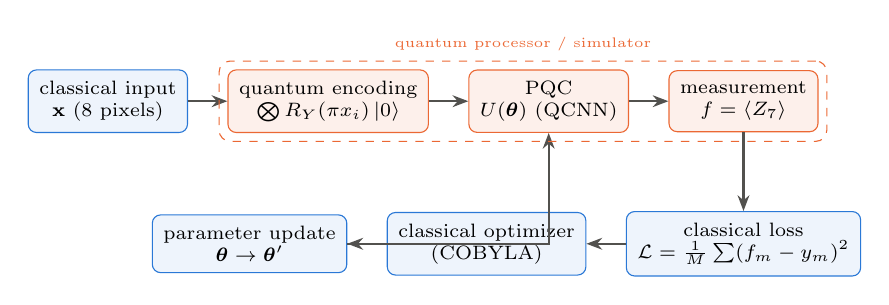
\begin{tikzpicture}[node distance=4mm and 5mm]
    \node[box] (in) {classical input\\$\bx$ (8 pixels)};
    \node[qbox, right=of in] (enc) {quantum encoding\\$\bigotimes R_Y(\pi x_i)\ket0$};
    \node[qbox, right=of enc] (pqc) {PQC\\$U(\btheta)$ (QCNN)};
    \node[qbox, right=of pqc] (meas) {measurement\\$f = \langle Z_7\rangle$};
    \node[box, below=10mm of meas] (loss) {classical loss\\$\mathcal L = \frac1M\sum(f_m - y_m)^2$};
    \node[box, left=of loss] (opt) {classical optimizer\\(COBYLA)};
    \node[box, left=of opt] (upd) {parameter update\\$\btheta \to \btheta'$};
    \draw[arr] (in) -- (enc); \draw[arr] (enc) -- (pqc); \draw[arr] (pqc) -- (meas); \draw[arr] (meas) -- (loss);
    \draw[arr] (loss) -- (opt); \draw[arr] (opt) -- (upd); \draw[arr] (upd) -| (pqc);
    \node[draw=qorange, dashed, rounded corners, fit=(enc)(pqc)(meas), inner sep=3pt, label={[font=\tiny, qorange]above:quantum processor / simulator}] {};
  \end{tikzpicture}\\[4pt]
  \begin{columns}[T]
    \begin{column}{0.5\textwidth}
      \scriptsize
      \begin{enumerate}\itemsep0pt
        \item scale the features to angles and prepare $\ket{\psi(\bx_m)}$;
        \item apply $U(\btheta)$ and estimate $f(\bx_m;\btheta)$ (exactly on a simulator, from shots on hardware);
        \item repeat for all $M$ images and compute $\mathcal L(\btheta)$ classically;
        \item the optimizer proposes new $\btheta$; repeat until the budget is used.
      \end{enumerate}
    \end{column}
    \begin{column}{0.46\textwidth}
      \scriptsize \key{Cost per loss evaluation}: $M$ circuits. Notebook: $100 \times 20 + 20 = 2020$ circuits, $\approx 1.7$ ms each on \texttt{qpp-cpu}
      $\Rightarrow \approx 3.4$ s (recorded).
    \end{column}
  \end{columns}
\end{frame}

\begin{frame}[label=fLossOut]{Loss, measurement and the classifier output}
  \begin{columns}[T]
    \begin{column}{0.52\textwidth}
      \small
      The quantum model returns an \key{expectation value} $f = \langle Z_{\text{out}}\rangle \in [-1, 1]$:
      \begin{itemize}\itemsep1pt
        \item prediction $\hat y = \operatorname{sign}f$ (decision boundary $f = 0$)
        \item margin $|f|$ = confidence
        \item loss $\mathcal L = \frac1M\sum(f_m - y_m)^2$, so a correct prediction with $|f| = 0.2$ still costs $(1 - 0.2)^2 = 0.64$
      \end{itemize}
      \begin{alertblock}{Recorded run}
        \scriptsize training MSE $\numfinalloss$ at training accuracy $\numtrainacc\,\%$: mean $|\langle Z_7\rangle| = \numtrainmargin$ --- correct signs, small margins.
      \end{alertblock}
    \end{column}
    \begin{column}{0.44\textwidth}
      \small Other read-outs:
      \begin{itemize}\itemsep1pt\scriptsize
        \item $p(y = 1) = \frac{1 + f}{2}$ with cross-entropy
        \item parity of several qubits, $\langle Z_0Z_1\rangle$
        \item one qubit per class, softmax over $\langle Z_k\rangle$
        \item trainable classical post-processing $w f + b$
      \end{itemize}
      \begin{block}{Measurement cost}
        \scriptsize On hardware $f$ is estimated from $S$ shots with error $\approx 1/\sqrt S$: margins of $0.2$ need well over 25 shots per image.
      \end{block}
    \end{column}
  \end{columns}
\end{frame}

\begin{frame}[label=fOpt]{Parameter optimization: gradient-free and gradient-based}
  \scriptsize
  \begin{center}
  \renewcommand{\arraystretch}{1.1}
  \resizebox{\linewidth}{!}{%
\begin{tabular}{p{3.2cm}p{5.0cm}p{5.0cm}}
    \toprule & \textbf{gradient-free} (COBYLA, Nelder--Mead, Powell, SPSA$^*$) & \textbf{gradient-based} (GD, Adam, L-BFGS)\\ \midrule
    needs & loss values only & $\nabla\mathcal L$: parameter shift or finite differences\\
    cost per step & 1 loss evaluation ($M$ circuits) & $\approx 2\times$(number of gate occurrences)$\times M$ circuits\\
    scaling with \#params & poor beyond a few dozen & good if gradients are cheap\\
    shot noise & COBYLA is sensitive; SPSA is designed for it & averages over many circuits\\
    in this repository & \texttt{QML.ipynb}: COBYLA (default), Nelder--Mead, Powell \tagimpl & L-BFGS-B with finite differences in \texttt{VQE.ipynb}, \texttt{QAOA.ipynb} \tagimpl\\ \bottomrule
  \end{tabular}}
  \end{center}
  {\scriptsize $^*$SPSA: simultaneous perturbation, 2 evaluations per step for any number of parameters (theory here).}
  \begin{exampleblock}{Cost of exact gradients for the 8-qubit QCNN}
    \scriptsize 11 convolution blocks $\times$ 2 $R_Y$ $\times$ 2 circuits $+$ 7 pooling blocks $\times$ 2 controlled rotations $\times$ 4 circuits
    $= 100$ circuits per image, $2000$ per gradient over 20 images --- as many as the whole COBYLA run.
  \end{exampleblock}
\end{frame}

\begin{frame}[label=fPSD]{The parameter-shift rule: derivation}
  \begin{columns}[T]
    \begin{column}{0.57\textwidth}
      \small
      Gate $G(\theta) = e^{-i\theta P/2}$ with $P^2 = I$ (a Pauli). Then $f(\theta) = a + b\cos\theta + c\sin\theta$, and
      \begin{align*}
        f(\theta + \tfrac\pi2) - f(\theta - \tfrac\pi2) &= b[\cos(\theta + \tfrac\pi2) - \cos(\theta - \tfrac\pi2)]\\
        &\quad + c[\sin(\theta + \tfrac\pi2) - \sin(\theta - \tfrac\pi2)]\\
        &= -2b\sin\theta + 2c\cos\theta = 2f'(\theta).
      \end{align*}
      \[ \boxed{\ f'(\theta) = \tfrac12\big[f(\theta + \tfrac\pi2) - f(\theta - \tfrac\pi2)\big]\ } \]
    \end{column}
    \begin{column}{0.40\textwidth}
      \begin{block}{Properties}
        \scriptsize
        \begin{itemize}\itemsep1pt
          \item \key{exact}: no step-size error (unlike finite differences)
          \item runs on hardware: two ordinary circuits
          \item shot noise remains: each $f$ is estimated
          \item \hl{only} for generators with two eigenvalues $\pm\frac12$; shared parameters need one shift pair \emph{per occurrence};
            controlled rotations need four terms
        \end{itemize}
      \end{block}
      \begin{exampleblock}{Numbers}
        \scriptsize $f(\theta + \frac\pi2) = 0.30$, $f(\theta - \frac\pi2) = -0.50$ $\Rightarrow$ $f'(\theta) = 0.40$.
      \end{exampleblock}
    \end{column}
  \end{columns}
\end{frame}

\begin{frame}[label=fPSC]{Parameter shift, checked with CUDA-Q \tagillus}
  \begin{columns}[T]
    \begin{column}{0.5\textwidth}
      \centering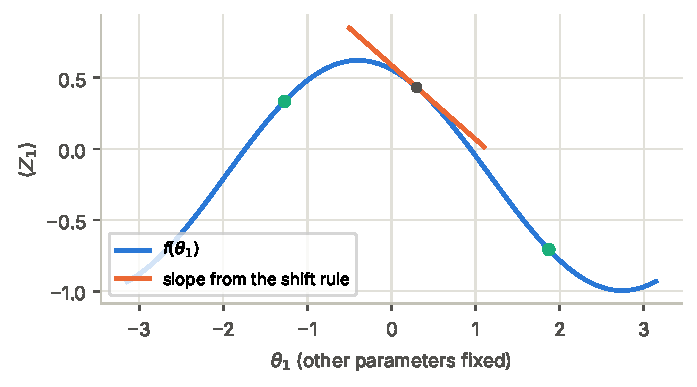
\includegraphics[width=\textwidth]{parameter_shift}\\
      {\scriptsize 2-qubit VQC: $R_Y(x_0)\otimes R_Y(x_1)$, $R_Y(\theta_1)\otimes R_Y(\theta_2)$, CNOT, $R_Y(\theta_3)$ on $q_1$; $f = \langle Z_1\rangle$; $\bx = (0.4, 1.1)$.}
    \end{column}
    \begin{column}{0.46\textwidth}
      \small
      At $\btheta = (0.3, -0.7, 0.5)$, two \texttt{cudaq.observe} calls per parameter give
      \[ \nabla f = (\numpsgradA,\ \numpsgradB,\ \numpsgradC). \]
      Largest difference from a central finite difference ($h = 10^{-5}$): $\numpserr$ --- the shift rule is exact.
      \begin{block}{Hybrid gradient of the loss}
        \scriptsize $\dfrac{\partial\mathcal L}{\partial\theta_k} = \dfrac1M\sum_m2(f_m - y_m)\,\dfrac{\partial f_m}{\partial\theta_k}$: quantum part by shift, classical part by the chain rule.
      \end{block}
    \end{column}
  \end{columns}
\end{frame}

\begin{frame}[label=fPSF]{When the two-term rule fails \tagillus}
  \begin{columns}[T]
    \begin{column}{0.52\textwidth}
      \small
      \key{Shared parameters}: in the QCNN, $\theta_{1,1}$ sits in 7 $R_Y$ gates, so $f$ contains frequencies up to 7 in it.
      \key{Controlled rotations}: generator $\ket1\!\bra1\otimes\frac P2$ has eigenvalues $0, \pm\frac12$ (frequencies $\frac12$, $1$).\\[3pt]
      Naive two-term rule on the \emph{trained} QCNN, first training image:
      \begin{center}\scriptsize
      % GENERATED by make_figures.py - do not edit
\begin{tabular}{lcc}\toprule
parameter & exact $\partial f$ & two-term shift \\ \midrule
$\theta_{1,1}$ (shared $R_Y$) & $+0.2890$ & $+0.0094$ \\
$\theta_{1,3}$ (controlled $R_Z$) & $-0.0055$ & $+0.0945$ \\
$\theta_{1,4}$ (controlled $R_X$) & $-0.0997$ & $-0.0089$ \\
\bottomrule
\end{tabular}

      \end{center}
    \end{column}
    \begin{column}{0.44\textwidth}
      \begin{block}{Four-term rule (controlled rotations)}
        \scriptsize
        \vspace{-6pt}
        \begin{align*}f' &= d_+\big[f(\theta + \tfrac\pi2) - f(\theta - \tfrac\pi2)\big]\\ &\ - d_-\big[f(\theta + \tfrac{3\pi}2) - f(\theta - \tfrac{3\pi}2)\big],\end{align*}
        \vspace{-8pt}\\ $d_\pm = \frac{\sqrt2 \pm 1}{4\sqrt2}$.
      \end{block}
      \begin{exampleblock}{Hadamard test, $f(\theta) = \cos\frac\theta2$, $\theta = 0.9$}
        \scriptsize exact $\numcrzfd$; two-term $\numcrztwo$ (wrong); four-term $\numcrzfour$ (exact).
      \end{exampleblock}
      \scriptsize Correct recipe for the QCNN: shift every occurrence separately and add (product rule).
    \end{column}
  \end{columns}
\end{frame}

% =====================================================================================
\section{Part D: QML algorithms}
\begin{frame}[label=fVQC]{Variational Quantum Classifier (VQC) \tagtheory}
  \begin{columns}[T]
    \begin{column}{0.52\textwidth}
      \small
      \key{Idea}: feature map $\to$ trainable ansatz $\to$ measure one observable $\to$ threshold.
      \[ f(\bx;\btheta) = \braket{\psi(\bx)|U^\dagger(\btheta)\,M\,U(\btheta)|\psi(\bx)}, \]
      \[ \hat y = \operatorname{sign}\big(f(\bx;\btheta) + b\big). \]
      Trained by minimising MSE / cross-entropy with a classical optimizer. The QCNN of the notebook is a VQC with a special ansatz;
      a general VQC with an entangling feature map is \emph{not} in this repository.
      \begin{itemize}\itemsep0pt\scriptsize
        \item use: small classification tasks, quantum data
        \item limits: trainability, shot cost, no proven advantage on classical data
      \end{itemize}
    \end{column}
    \begin{column}{0.44\textwidth}
      \begin{center}
      \begin{quantikz}[row sep=0.25cm, column sep=0.3cm]
        \lstick{$\ket0$} & \gate{R_Y(x_0)} & \ctrl{1} & \qw & \qw \\
        \lstick{$\ket0$} & \gate{R_Y(x_1)} & \targ{} & \gate{R_Y(\theta)} & \meter{}
      \end{quantikz}
      \end{center}
      \begin{exampleblock}{Worked example (Heisenberg picture)}
        \scriptsize $Z_1 \xrightarrow{R_Y(\theta)} \cos\theta Z_1 - \sin\theta X_1 \xrightarrow{\text{CNOT}} \cos\theta Z_0Z_1 - \sin\theta X_1$:\\
        $f = \cos\theta\cos x_0\cos x_1 - \sin\theta\sin x_1$.\\
        $\bx = (0, \frac\pi3)$, $\theta = \frac\pi6$: $f = 0$; $f(\theta \pm \frac\pi2) = \mp1$; $f' = -1$;
        $y = +1$: $\partial_\theta(f - y)^2 = 2(0 - 1)(-1) = 2$.
      \end{exampleblock}
    \end{column}
  \end{columns}
\end{frame}

\begin{frame}[label=fQSVM]{Quantum SVM and kernel methods \tagtheory}
  \begin{columns}[T]
    \begin{column}{0.52\textwidth}
      \small
      \key{SVM}: find the maximum-margin separator in feature space. Dual problem (only kernels appear):
      \[ \max_{\boldsymbol\alpha}\ \sum_m\alpha_m - \tfrac12\sum_{m,m'}\alpha_m\alpha_{m'}y_my_{m'}k(\bx_m, \bx_{m'}) \]
      subject to $0 \le \alpha_m \le C$, $\sum_m\alpha_my_m = 0$. Prediction: $\hat y = \operatorname{sign}\big(\sum_m\alpha_my_mk(\bx_m, \bx) + b\big)$.\\[3pt]
      \key{Quantum SVM}: the quantum computer only estimates $k$; the optimisation is a classical convex QP --- no barren plateaus.
    \end{column}
    \begin{column}{0.44\textwidth}
      \begin{block}{Strengths and limits}
        \scriptsize
        \begin{itemize}\itemsep1pt
          \item convex training, guaranteed optimum
          \item $O(M^2)$ kernel circuits, each with many shots
          \item kernel values concentrate exponentially for many features (Part E) $\Rightarrow$ poor generalisation
          \item a kernel that is classically computable gives no quantum advantage
        \end{itemize}
      \end{block}
      \scriptsize Havlíček et al., \emph{Nature} 567 (2019); Schuld \& Killoran, PRL 122 (2019).
    \end{column}
  \end{columns}
\end{frame}

\begin{frame}[label=fKSVM]{Quantum-kernel SVM on the notebook's data \tagillus}
  \begin{columns}[T]
    \begin{column}{0.38\textwidth}
      \centering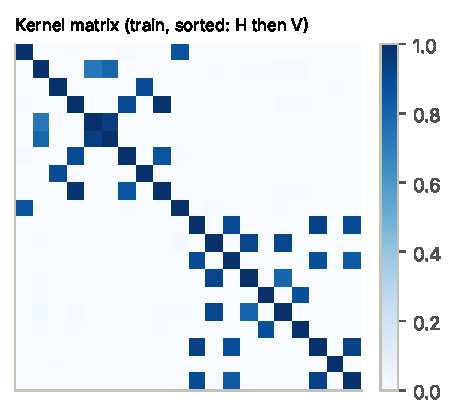
\includegraphics[width=\textwidth]{kernel_matrix}
    \end{column}
    \begin{column}{0.58\textwidth}
      \small
      Feature map = the notebook's angle encoding; kernel from CUDA-Q states (\texttt{cudaq.get\_state}); SVM dual solved classically ($C = 10$).
      \begin{itemize}\itemsep1pt
        \item CUDA-Q kernel = analytic $\prod\cos^2$ formula to $\numkerndiff$
        \item mean off-diagonal kernel value $\numkmean$ (8 features already push $k$ towards 0)
        \item \numsvmsv{} support vectors of 20; training accuracy \numsvmtrain\,\%, test accuracy \numsvmtest\,\%
        \item 2000 fresh images: \numsvmbig\,\% (QCNN: \numbigacc\,\%)
      \end{itemize}
      \begin{alertblock}{Interpretation}
        \scriptsize A better classifier than the QCNN here --- but its kernel is a cheap classical formula, so this is \emph{not} a quantum advantage.
      \end{alertblock}
    \end{column}
  \end{columns}
\end{frame}

\begin{frame}[label=fQCNN]{QNN and the Quantum Convolutional Neural Network \tagimpl}
  \begin{columns}[T]
    \begin{column}{0.42\textwidth}
      \small
      QCNN (Cong, Choi \& Lukin, \emph{Nat.\ Phys.}\ 2019):
      \begin{itemize}\itemsep1pt
        \item \key{convolution}: the same 2-qubit block on all neighbouring pairs (shared weights)
        \item \key{pooling}: a controlled rotation passes information from a source to a sink; the source is discarded
        \item repeat until one qubit is left: $\lceil\log_2N\rceil$ layers, $O(\log N)$ parameters
        \item provably free of barren plateaus (Pesah et al., PRX 2021)
      \end{itemize}
    \end{column}
    \begin{column}{0.56\textwidth}
      \centering
      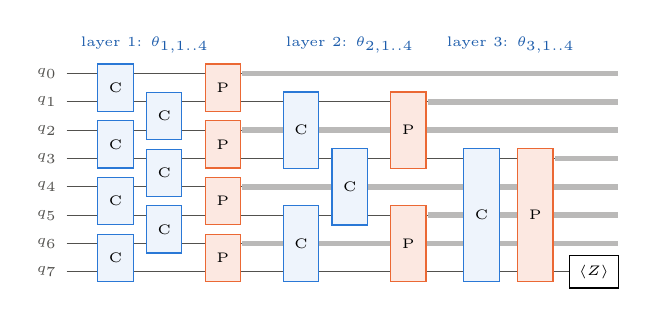
\begin{tikzpicture}[x=0.62cm, y=0.36cm]
        \foreach \q in {0,...,7} {\draw[qgrey] (0,-\q) node[left, font=\tiny]{$q_\q$} -- (11.3,-\q);}
        % layer 1
        \foreach \a in {0,2,4,6} {\node[draw=qblue, fill=qlight, minimum width=0.45cm, minimum height=0.6cm, inner sep=0] at (1,-\a-0.5) {\tiny C};}
        \foreach \a in {1,3,5} {\node[draw=qblue, fill=qlight, minimum width=0.45cm, minimum height=0.6cm, inner sep=0] at (2,-\a-0.5) {\tiny C};}
        \foreach \a in {0,2,4,6} {\node[draw=qorange, fill=qorange!15, minimum width=0.45cm, minimum height=0.6cm, inner sep=0] at (3.2,-\a-0.5) {\tiny P};}
        \foreach \a in {0,2,4,6} {\draw[qgrey!40, line width=2pt] (3.6,-\a) -- (11.3,-\a);}
        % layer 2: active 1,3,5,7
        \foreach \a/\b in {1/3,5/7} {\node[draw=qblue, fill=qlight, minimum width=0.45cm, minimum height=0.36cm*(\b-\a)+0.25cm, inner sep=0] at (4.8,-\a/2-\b/2) {\tiny C};}
        \node[draw=qblue, fill=qlight, minimum width=0.45cm, minimum height=0.97cm, inner sep=0] at (5.8,-4) {\tiny C};
        \foreach \a/\b in {1/3,5/7} {\node[draw=qorange, fill=qorange!15, minimum width=0.45cm, minimum height=0.36cm*(\b-\a)+0.25cm, inner sep=0] at (7,-\a/2-\b/2) {\tiny P};}
        \foreach \a in {1,5} {\draw[qgrey!40, line width=2pt] (7.4,-\a) -- (11.3,-\a);}
        % layer 3: active 3,7
        \node[draw=qblue, fill=qlight, minimum width=0.45cm, minimum height=1.69cm, inner sep=0] at (8.5,-5) {\tiny C};
        \node[draw=qorange, fill=qorange!15, minimum width=0.45cm, minimum height=1.69cm, inner sep=0] at (9.6,-5) {\tiny P};
        \draw[qgrey!40, line width=2pt] (10,-3) -- (11.3,-3);
        \node[draw, fill=white, font=\tiny] at (10.8,-7) {$\langle Z\rangle$};
        \node[font=\tiny, qdark] at (1.6,1) {layer 1: $\theta_{1,1..4}$}; \node[font=\tiny, qdark] at (5.8,1) {layer 2: $\theta_{2,1..4}$};
        \node[font=\tiny, qdark] at (9.1,1) {layer 3: $\theta_{3,1..4}$};
      \end{tikzpicture}\\
      {\scriptsize 8 qubits $\to$ 4 $\to$ 2 $\to$ 1. C = convolution block, P = pooling block (grey = discarded qubit). Output: qubit 7.}
    \end{column}
  \end{columns}
\end{frame}

\begin{frame}[label=fBlocks]{QCNN building blocks (\texttt{QML.ipynb})}
  \begin{columns}[T]
    \begin{column}{0.48\textwidth}
      \begin{block}{Convolution block on $(a, b)$, layer $\ell$}
        \centering
        \begin{quantikz}[row sep=0.25cm, column sep=0.35cm]
          \lstick{$a$} & \gate{R_Y(\theta_{\ell,1})} & \ctrl{1} & \qw \\
          \lstick{$b$} & \gate{R_Y(\theta_{\ell,2})} & \targ{} & \qw
        \end{quantikz}\\
        \scriptsize $U_\ell = \mathrm{CNOT}_{a\to b}\big(R_Y(\theta_{\ell,1})\otimes R_Y(\theta_{\ell,2})\big)$, on pairs $(0,1), (2,3), \dots$ then $(1,2), (3,4), \dots$
      \end{block}
    \end{column}
    \begin{column}{0.48\textwidth}
      \begin{block}{Pooling block, source $a$ $\to$ sink $b$}
        \centering
        \begin{quantikz}[row sep=0.25cm, column sep=0.3cm]
          \lstick{$a$} & \ctrl{1} & \gate{X} & \ctrl{1} & \gate{X} & \qw \\
          \lstick{$b$} & \gate{R_Z(\theta_{\ell,3})} & \qw & \gate{R_X(\theta_{\ell,4})} & \qw & \qw
        \end{quantikz}\\
        \scriptsize $P_\ell = \ket1\!\bra1_a\otimes R_Z(\theta_{\ell,3}) + \ket0\!\bra0_a\otimes R_X(\theta_{\ell,4})$
      \end{block}
    \end{column}
  \end{columns}
  \small
  \begin{itemize}\itemsep1pt
    \item The $X\cdots X$ sandwich turns the second controlled gate into an \emph{anti}-controlled one (acts when $a = 0$).
    \item \key{Deferred measurement}: ``measure $a$, then rotate $b$ depending on the result'' $=$ controlled rotation, then ignore $a$ --- no mid-circuit measurement needed.
    \item Gate count: $N + 3n_{\text{conv}} + 4n_{\text{pool}}$; $N = 8$: $8 + 33 + 28 = \numngates$ gates, depth \numdepth.
  \end{itemize}
\end{frame}

\begin{frame}[label=fSize]{QCNN size versus number of qubits \tagimpl}
  \begin{columns}[T]
    \begin{column}{0.52\textwidth}
      \footnotesize
      \begin{center}
      % GENERATED by make_figures.py - do not edit
\begin{tabular}{rrrrrr}\toprule
$N$ & layers & params & conv & pool & output \\ \midrule
4 & 2 & 8 & 4 & 3 & 3 \\
8 & 3 & 12 & 11 & 7 & 7 \\
15 & 4 & 16 & 25 & 14 & 14 \\
16 & 4 & 16 & 26 & 15 & 15 \\
20 & 5 & 20 & 35 & 19 & 19 \\
30 & 5 & 20 & 54 & 29 & 29 \\
\bottomrule
\end{tabular}

      \end{center}
      {\scriptsize computed with the notebook's \texttt{qcnn\_layout}; layers $= \lceil\log_2N\rceil$.}
    \end{column}
    \begin{column}{0.44\textwidth}
      \small
      \begin{itemize}\itemsep1pt
        \item pooling keeps $\lceil n/2\rceil$: $20 \to 10 \to 5 \to 3 \to 2 \to 1$
        \item parameters grow \emph{logarithmically}: 12 at $N = 8$, 20 at $N = 30$
        \item gates grow \emph{linearly}: $N = 16$: $16 + 3\cdot26 + 4\cdot15 = 154$
        \item the classical simulation cost grows \emph{exponentially} ($2^N$)
      \end{itemize}
    \end{column}
  \end{columns}
\end{frame}

\begin{frame}[label=fGAN]{Quantum Generative Adversarial Networks \tagtheory}
  \begin{columns}[T]
    \begin{column}{0.5\textwidth}
      \small
      A \key{generator} $G$ produces samples; a \key{discriminator} $D$ tries to tell them from real data.
      \[ \min_G\max_D\ \mathbb E_{\text{data}}[\ln D(x)] + \mathbb E_{G}[\ln(1 - D(x))]. \]
      Quantum GAN: $G$ is a PQC whose measurement distribution $p_{\btheta}(x) = |\braket{x|U(\btheta)|0}|^2$ is the model; $D$ may be classical or quantum.
      At equilibrium $p_G = p_{\text{data}}$, $D = \frac12$, value $-\ln4$.
    \end{column}
    \begin{column}{0.46\textwidth}
      \centering
      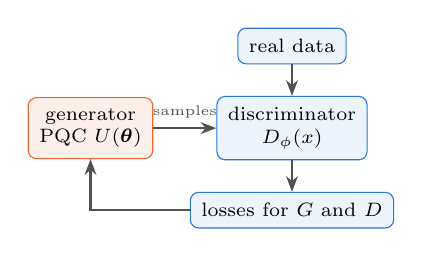
\begin{tikzpicture}[node distance=4mm]
        \node[qbox] (g) {generator\\PQC $U(\btheta)$};
        \node[box, right=8mm of g] (d) {discriminator\\$D_\phi(x)$};
        \node[box, above=of d] (r) {real data};
        \node[box, below=of d] (l) {losses for $G$ and $D$};
        \draw[arr] (g) -- node[above, font=\tiny]{samples} (d); \draw[arr] (r) -- (d); \draw[arr] (d) -- (l);
        \draw[arr] (l) -| (g);
      \end{tikzpicture}
      \begin{block}{Uses and limits}
        \scriptsize loading distributions (e.g.\ for finance), learning quantum states. Training is unstable (as for classical GANs); sampling cost; no general advantage shown.
      \end{block}
    \end{column}
  \end{columns}
\end{frame}

\begin{frame}[label=fPCA]{Quantum Principal Component Analysis \tagtheory}
  \begin{columns}[T]
    \begin{column}{0.52\textwidth}
      \small
      Lloyd, Mohseni \& Rebentrost (\emph{Nat.\ Phys.}\ 2014):
      \begin{enumerate}\itemsep1pt
        \item prepare many copies of the (normalised) covariance matrix as a density matrix $\rho$
        \item simulate $e^{-i\rho t}$ by repeated partial SWAPs with fresh copies (density-matrix exponentiation)
        \item phase estimation $\Rightarrow$ $\sum_k\sqrt{\lambda_k}\ket{v_k}\ket{\tilde\lambda_k}$: large eigenvalues and eigenvectors \emph{as quantum states}
      \end{enumerate}
      Cost polylogarithmic in the dimension --- for low-rank $\rho$ and efficient state access.
    \end{column}
    \begin{column}{0.44\textwidth}
      \begin{alertblock}{Caveats}
        \scriptsize
        \begin{itemize}\itemsep1pt
          \item reading out an eigenvector classically costs its dimension
          \item needs QRAM-like data access
          \item ``dequantized'' classical sampling algorithms (Tang 2019; Chia et al.\ 2020) reach polylog scaling for low-rank PCA under comparable access
          \item needs fault-tolerant hardware (phase estimation)
        \end{itemize}
      \end{alertblock}
      \scriptsize Classical PCA example: $C = \begin{psmallmatrix}2&1\\1&2\end{psmallmatrix}$, $\lambda = 3, 1$, first component $(1,1)/\sqrt2$ explains $75\,\%$.
    \end{column}
  \end{columns}
\end{frame}

\begin{frame}[label=fClusRL]{Quantum clustering and quantum reinforcement learning \tagtheory}
  \begin{columns}[T]
    \begin{column}{0.5\textwidth}
      \begin{block}{Clustering}
        \scriptsize
        \key{$k$-means}: assign points to the nearest centroid, update centroids. Quantum versions (q-means, Kerenidis et al.\ 2019) estimate distances
        with overlap circuits:
        \[ \|\mathbf a - \mathbf b\|^2 = 2 - 2\,\mathbf a\cdot\mathbf b,\quad |\mathbf a\cdot\mathbf b|^2 = 2P_{\text{swap}}(0) - 1. \]
        Example: $P(0) = 0.9 \Rightarrow \mathbf a\cdot\mathbf b = \sqrt{0.8} = 0.894$, distance $0.46$.
        Kernel-based clustering can use quantum kernels. Same caveats: data access, shot cost, dequantization.
      \end{block}
    \end{column}
    \begin{column}{0.46\textwidth}
      \begin{block}{Reinforcement learning}
        \scriptsize
        An agent in state $s$ takes action $a$, gets reward $r$. Q-learning:
        \[ Q(s,a) \leftarrow Q + \alpha\big[r + \gamma\max_{a'}Q(s',a') - Q\big]. \]
        $Q = 2$, $\alpha = 0.5$, $r = 1$, $\gamma = 0.9$, $\max Q' = 4$: $Q \to 3.3$.\\[2pt]
        Quantum RL: a PQC represents the policy $\pi(a\mid s) = |\braket{a|U(s;\btheta)|0}|^2$ or the Q-function (Jerbi et al.\ 2021; Skolik et al.\ 2022);
        speed-ups proven only for specially constructed environments.
      \end{block}
    \end{column}
  \end{columns}
\end{frame}

\begin{frame}[label=fQData]{Quantum data classification}
  \begin{columns}[T]
    \begin{column}{0.52\textwidth}
      \small
      The original QCNN task: given a quantum state $\ket\psi$ produced by a physical system, decide its \key{phase} (e.g.\ symmetry-protected
      topological vs.\ trivial).
      \begin{itemize}\itemsep1pt
        \item no encoding cost: the data are already quantum
        \item the classical alternative must first learn the state from measurements (tomography: exponential in general)
        \item here quantum models have provable sample-complexity advantages for some tasks (Huang et al., \emph{Science} 2022)
      \end{itemize}
    \end{column}
    \begin{column}{0.44\textwidth}
      \begin{block}{\texttt{QML.ipynb} by contrast}
        \scriptsize classifies \emph{classical} images (horizontal vs.\ vertical lines) that are angle-encoded --- a teaching example of the
        architecture, explicitly not intended to beat classical methods (notebook, Section 1).
      \end{block}
      \begin{alertblock}{Take-away}
        \scriptsize The most credible routes to quantum advantage in ML involve \key{quantum data}, not small classical datasets.
      \end{alertblock}
    \end{column}
  \end{columns}
\end{frame}

% =====================================================================================
\section{Part E: Advanced QML and implementation}
\begin{frame}[label=fHArch]{Hybrid quantum--classical architectures}
  \begin{columns}[T]
    \begin{column}{0.52\textwidth}
      \small
      \begin{itemize}\itemsep2pt
        \item \key{quantum layer in a classical network}: classical pre-processing (e.g.\ CNN features, PCA to $n$ numbers) $\to$ PQC $\to$ classical head
        \item \key{quantum feature extractor}: measure many observables, train a classical model on them
        \item \key{quantum kernel + classical SVM}
        \item \key{end-to-end PQC} with classical optimizer --- the design of \texttt{QML.ipynb}
      \end{itemize}
      \scriptsize Frameworks connect CUDA-Q kernels to PyTorch-style autodiff by supplying gradients from parameter shift or adjoint simulation.
    \end{column}
    \begin{column}{0.44\textwidth}
      \centering
      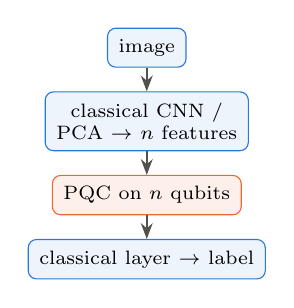
\begin{tikzpicture}[node distance=3mm]
        \node[box] (a) {image};
        \node[box, below=of a] (b) {classical CNN /\\PCA $\to$ $n$ features};
        \node[qbox, below=of b] (c) {PQC on $n$ qubits};
        \node[box, below=of c] (d) {classical layer $\to$ label};
        \draw[arr] (a) -- (b); \draw[arr] (b) -- (c); \draw[arr] (c) -- (d);
      \end{tikzpicture}\\
      \scriptsize With such pipelines it is essential to check how much of the accuracy comes from the classical parts.
    \end{column}
  \end{columns}
\end{frame}

\begin{frame}[label=fBP]{Barren plateaus and vanishing gradients}
  \begin{columns}[T]
    \begin{column}{0.52\textwidth}
      \small
      \key{Barren plateau}: for random parameters $\mathbb E[\partial_kC] = 0$ and
      \[ \operatorname{Var}[\partial_kC] \in O(b^{-n}),\ b > 1. \]
      By Chebyshev, gradients larger than $\epsilon$ are exponentially rare; resolving them needs $\sim b^n$ shots.
      \begin{itemize}\itemsep1pt\scriptsize
        \item deep random circuits (2-designs): McClean et al., \emph{Nat.\ Commun.}\ 2018
        \item global costs even in shallow circuits: Cerezo et al., \emph{Nat.\ Commun.}\ 2021
        \item noise-induced plateaus: Wang et al., \emph{Nat.\ Commun.}\ 2021
        \item gradient-free optimizers are affected too (Arrasmith et al.\ 2021)
      \end{itemize}
    \end{column}
    \begin{column}{0.44\textwidth}
      \begin{block}{Mitigations}
        \scriptsize
        \begin{itemize}\itemsep1pt
          \item local cost functions, shallow circuits
          \item structured ans\"atze with few parameters (QCNN: no barren plateau, Pesah et al.\ 2021)
          \item small-angle / identity-block initialisation, layer-wise training
          \item caution: architectures provably free of plateaus are often classically simulable (Cerezo et al.\ 2023)
        \end{itemize}
      \end{block}
    \end{column}
  \end{columns}
\end{frame}

\begin{frame}[label=fBPm]{Barren plateaus, measured with CUDA-Q \tagillus}
  \begin{columns}[T]
    \begin{column}{0.56\textwidth}
      \centering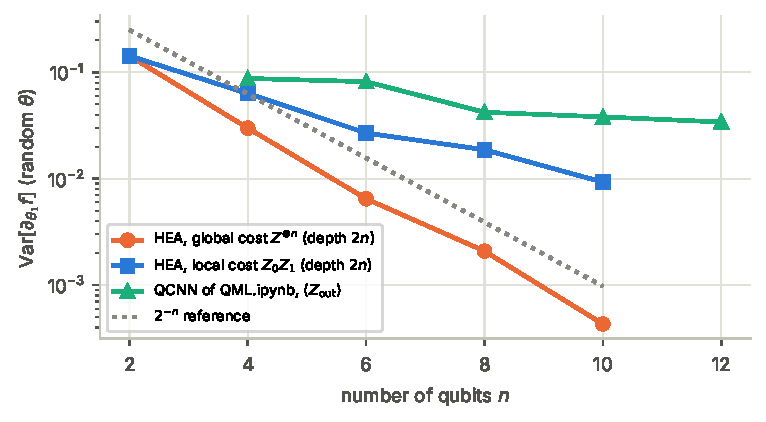
\includegraphics[width=\textwidth]{barren_plateau}
    \end{column}
    \begin{column}{0.40\textwidth}
      \small
      Variance of $\partial f/\partial\theta_1$ over random parameters (200 samples per point; QCNN: 100, random pixels):
      \begin{itemize}\itemsep1pt\scriptsize
        \item HEA, depth $2n$, global $Z^{\otimes n}$: falls roughly like $2^{-n}$ (\numvarglobten{} at $n = 10$)
        \item same circuit, local $Z_0Z_1$: decays more slowly (\numvarlocten)
        \item QCNN of \texttt{QML.ipynb}: \numvarqcnntwelve{} at $n = 12$
      \end{itemize}
      \scriptsize Small sizes only (CPU simulation); a trend, not a proof.
    \end{column}
  \end{columns}
\end{frame}

\begin{frame}[label=fExpr]{Expressibility, entanglement, depth and trainability}
  \begin{columns}[T]
    \begin{column}{0.52\textwidth}
      \small
      \begin{itemize}\itemsep2pt
        \item \key{Expressibility}: how much of the state space an ansatz can reach (Sim et al.\ 2019). More expressive ans\"atze have flatter landscapes
          (Holmes et al.\ 2022): a trade-off.
        \item \key{Entanglement}: needed for non-trivial models, but too much entanglement makes local observables uninformative (Part B example).
        \item \key{Depth}: more layers $\Rightarrow$ more expressive, more noise, more plateau-prone; parameter count also grows.
        \item \key{Inductive bias}: an architecture matched to the data (translation invariance $\to$ QCNN) beats generic expressivity.
      \end{itemize}
    \end{column}
    \begin{column}{0.44\textwidth}
      \begin{block}{The notebook's QCNN}
        \scriptsize
        \begin{itemize}\itemsep1pt
          \item depth \numdepth{} (8 qubits), only $\numnparams$ shared parameters
          \item log-depth in layers, local structure
          \item README: a 15-qubit run with 60 COBYLA evaluations reached only 69\,\% --- deeper models need more optimizer steps
        \end{itemize}
      \end{block}
    \end{column}
  \end{columns}
\end{frame}

\begin{frame}[label=fNoise]{Noise in QML \tagillus}
  \begin{columns}[T]
    \begin{column}{0.48\textwidth}
      \small
      Real devices apply noise channels, e.g.\ depolarising $\rho \mapsto (1 - p)\rho + p\frac I2$ after gates. Effects:
      \begin{itemize}\itemsep1pt
        \item expectation values shrink towards 0; a simple model gives $(1 - p)^G$: $0.99^{69} \approx 0.50$
        \item signs (predictions) survive longer than margins
        \item noise can flatten landscapes (noise-induced plateaus)
      \end{itemize}
      \scriptsize Measured: trained QCNN, 20 test images, depolarising channels after every gate (\texttt{density-matrix-cpu}).
    \end{column}
    \begin{column}{0.48\textwidth}
      \footnotesize
      \begin{center}
      % GENERATED by make_figures.py - do not edit
\begin{tabular}{rccc}\toprule
$p$ & accuracy & mean $|\langle Z\rangle|$ & MSE \\ \midrule
0 & 85\,\% & 0.171 & 0.725 \\
0.01 & 85\,\% & 0.112 & 0.809 \\
0.03 & 85\,\% & 0.047 & 0.913 \\
0.1 & 85\,\% & 0.003 & 0.995 \\
\bottomrule
\end{tabular}

      \end{center}
      \scriptsize Accuracy unchanged, but the margins collapse: at $p = 0.1$ the outputs ($\approx 0.003$) would need $\sim10^5$ shots per image to read their signs.
    \end{column}
  \end{columns}
\end{frame}

\begin{frame}[label=fShots]{Finite shots \tagillus}
  \begin{columns}[T]
    \begin{column}{0.5\textwidth}
      \small
      On hardware $\langle Z_7\rangle$ is estimated from $S$ shots. Test accuracy of the trained QCNN with \texttt{cudaq.observe(..., shots\_count=S)}, 5 repetitions:
      \begin{center}\footnotesize
      % GENERATED by make_figures.py - do not edit
\begin{tabular}{rccc}\toprule
$S$ & mean & range & $1/\sqrt S$ \\ \midrule
10 & 63\,\% & 60--70\,\% & 0.316 \\
100 & 86\,\% & 75--100\,\% & 0.100 \\
1,000 & 84\,\% & 80--90\,\% & 0.032 \\
10,000 & 83\,\% & 80--85\,\% & 0.010 \\
\bottomrule
\end{tabular}

      \end{center}
    \end{column}
    \begin{column}{0.46\textwidth}
      \begin{alertblock}{Why so many shots?}
        \scriptsize The mean $|\langle Z_7\rangle|$ on the test images is \numtestmargin: the statistical error must be well below that.
        Training with shots is harder still: COBYLA then sees a noisy loss.
      \end{alertblock}
      \scriptsize Exact (state-vector) accuracy: \numtestacc\,\%. Differences of a few points at large $S$ are sampling fluctuations of individual
      images with $|\langle Z\rangle| \ll 0.1$.
    \end{column}
  \end{columns}
\end{frame}

\begin{frame}[label=fBase]{Evaluating a quantum model: classical baselines \tagillus}
  \footnotesize
  \begin{center}
\resizebox{\linewidth}{!}{%
  \begin{tabular}{lccc}
    \toprule \textbf{Model (same 20 training images)} & \textbf{test, 20 images} & \textbf{2000 fresh images} & \textbf{trainable parameters}\\ \midrule
    QCNN of \texttt{QML.ipynb} (re-executed) & \numtestacc\,\% & \numbigacc\,\% & \numnparams\\
    logistic regression on the 8 pixels & \numlrtest\,\% & \numbiglr\,\% & \numlrparams\\
    SVM, kernel of the notebook's angle encoding & \numsvmtest\,\% & \numsvmbig\,\% & 20 dual coefficients\\
    hand-made rule (brightest pair) & \numruletest\,\% & \numbigrule\,\% & 0\\ \bottomrule
  \end{tabular}}
  \end{center}
  \begin{columns}[T]
    \begin{column}{0.5\textwidth}
      \scriptsize
      \begin{itemize}\itemsep1pt
        \item Logistic regression fails: the clean images are \emph{not linearly separable} (the two middle horizontal pairs and the two middle vertical lines
          light the same four pixels).
        \item The QCNN is non-linear in the pixels and does learn, but generalises worse than the classically computable kernel SVM.
      \end{itemize}
    \end{column}
    \begin{column}{0.46\textwidth}
      \begin{alertblock}{Conclusion}
        \scriptsize No quantum advantage on this task. The notebook's goal is to teach the QCNN, not to beat classical methods --- and it says so.
      \end{alertblock}
    \end{column}
  \end{columns}
\end{frame}

\begin{frame}[fragile,label=fData]{Dataset preprocessing and the training/testing pipeline \tagimpl}
  \begin{columns}[T]
    \begin{column}{0.55\textwidth}
\begin{lstlisting}[basicstyle=\ttfamily\tiny]
rng = np.random.default_rng(SEED)
def make_images(count):
    images, labels = [], []
    for k in range(count):
        image = rng.uniform(0, NOISE_LEVEL,
                            size=(IMAGE_ROWS, IMAGE_COLS))
        if k % 2 == 0:                       # horizontal
            row = rng.integers(IMAGE_ROWS)
            col = rng.integers(IMAGE_COLS - LINE_LENGTH + 1)
            image[row, col:col + LINE_LENGTH] = 1.0
            labels.append(+1)
        else:                                # vertical
            col = rng.integers(IMAGE_COLS)
            row = rng.integers(IMAGE_ROWS - LINE_LENGTH + 1)
            image[row:row + LINE_LENGTH, col] = 1.0
            labels.append(-1)
        images.append(image.ravel())         # pixel -> qubit
    return np.array(images), np.array(labels)
\end{lstlisting}
    \end{column}
    \begin{column}{0.42\textwidth}
      \scriptsize
      \begin{itemize}\itemsep1pt
        \item synthetic data: dark background in $[0, 0.25]$, one line of 2 pixels $= 1.0$
        \item classes alternate $\Rightarrow$ exactly balanced
        \item values already in $[0, 1]$: no further scaling; angle $= \pi x$
        \item \texttt{ravel()}: row-major flattening, pixel $(r, c) \to$ qubit $4r + c$
        \item train and test: two consecutive calls on one generator, seed 42 $\Rightarrow$ reproducible, independent
        \item own data: any array of shape $(M, N)$ in $[0, 1]$ with labels $\pm1$
      \end{itemize}
    \end{column}
  \end{columns}
\end{frame}

\begin{frame}[fragile,label=fStruct]{The structure of \texttt{QML.ipynb}}
  \begin{columns}[T]
    \begin{column}{0.53\textwidth}
      \scriptsize
      \begin{tabular}{rl}
        \toprule \textbf{Section} & \textbf{Content}\\ \midrule
        1 & problem statement and mathematics\\
        2 & imports, versions, number of GPUs\\
        3 & \key{input parameters} (the only cell to edit)\\
        4 & image dataset (\texttt{make\_images})\\
        5 & target, \texttt{qcnn\_layout}, kernel, drawing, resources\\
        6 & expected output, time per circuit, memory\\
        7 & training (execution cell)\\
        8 & plots: curves, gallery, histogram\\
        9 & final report\\ \bottomrule
      \end{tabular}\\[3pt]
      \scriptsize Generated by \texttt{dev/notebook\_builders/build\_qml.py}; deliberately short, without the shared monitoring utilities of the other notebooks.
    \end{column}
    \begin{column}{0.45\textwidth}
\begin{lstlisting}[basicstyle=\ttfamily\tiny]
IMAGE_ROWS = 2;  IMAGE_COLS = 4   # N = 8 qubits
LINE_LENGTH = 2; NOISE_LEVEL = 0.25
TRAIN_IMAGES = 20; TEST_IMAGES = 20
OPTIMIZER = "COBYLA"; MAX_ITERATIONS = 100
INITIAL_PARAMETER_SCALE = 3.14
TARGET = "auto"; SEED = 42
N_QUBITS = IMAGE_ROWS * IMAGE_COLS
\end{lstlisting}
      \scriptsize \texttt{TARGET = "auto"}: \texttt{"nvidia"} if \texttt{cudaq.num\_available\_gpus() > 0}, else \texttt{"qpp-cpu"}.
      GPU targets are refused when no GPU is visible.
    \end{column}
  \end{columns}
\end{frame}

\begin{frame}[fragile,label=fLayout]{The layout function, line by line (Section 5)}
  \begin{columns}[T]
    \begin{column}{0.57\textwidth}
\begin{lstlisting}[basicstyle=\ttfamily\tiny]
def qcnn_layout(n):
    kinds, qubit_a, qubit_b, layers = [], [], [], []
    active, layer = list(range(n)), 0
    while len(active) > 1:
        for start in (0, 1):                 # conv pairs
            for i in range(start, len(active) - 1, 2):
                kinds.append(0); qubit_a.append(active[i])
                qubit_b.append(active[i + 1]); layers.append(layer)
        kept = []
        for i in range(0, len(active) - 1, 2):   # pooling
            kinds.append(1); qubit_a.append(active[i])
            qubit_b.append(active[i + 1]); layers.append(layer)
            kept.append(active[i + 1])       # sink survives
        if len(active) % 2 == 1:
            kept.append(active[-1])          # odd qubit moves on
        active, layer = kept, layer + 1
    return kinds, qubit_a, qubit_b, layers, active[0], layer
\end{lstlisting}
    \end{column}
    \begin{column}{0.40\textwidth}
      \scriptsize
      \begin{itemize}\itemsep1pt
        \item plain Python, run once: a list of operations (kind, qubit $a$, qubit $b$, layer)
        \item \texttt{start = 0}: pairs $(0,1), (2,3), \dots$; \texttt{start = 1}: $(1,2), (3,4), \dots$ --- like a stride-2 convolution applied twice
        \item pooling: source \texttt{active[i]}, sink \texttt{active[i+1]}; sinks survive
        \item $N = 8$: layer 1: 7 conv + 4 pool on $\{0..7\}$; layer 2: 3 + 2 on $\{1,3,5,7\}$; layer 3: 1 + 1 on $\{3,7\}$
        \item result: \numnblocks{} blocks, \numnlayers{} layers, output qubit \numoutqubit
      \end{itemize}
    \end{column}
  \end{columns}
\end{frame}

\begin{frame}[fragile,label=fKernel]{The CUDA-Q kernel, line by line (Section 5)}
  \begin{columns}[T]
    \begin{column}{0.57\textwidth}
\begin{lstlisting}
@cudaq.kernel
def qcnn(pixels: list[float], theta: list[float],
         kinds: list[int], qubit_a: list[int],
         qubit_b: list[int], layers: list[int]):
    qubits = cudaq.qvector(len(pixels))   # |0...0>
    for i in range(len(pixels)):
        ry(np.pi * pixels[i], qubits[i])  # encoding
    for k in range(len(kinds)):
        t = 4 * layers[k]                 # theta[t..t+3]
        a = qubit_a[k]
        b = qubit_b[k]
        if kinds[k] == 0:                 # convolution
            ry(theta[t], qubits[a])
            ry(theta[t + 1], qubits[b])
            x.ctrl(qubits[a], qubits[b])
        else:                             # pooling a -> b
            rz.ctrl(theta[t + 2], qubits[a], qubits[b])
            x(qubits[a])
            rx.ctrl(theta[t + 3], qubits[a], qubits[b])
            x(qubits[a])
\end{lstlisting}
    \end{column}
    \begin{column}{0.40\textwidth}
      \scriptsize
      \begin{itemize}\itemsep1pt
        \item \texttt{@cudaq.kernel}: compiled (MLIR/QIR) and JIT-compiled on first call
        \item the kernel only \emph{walks} the operation list; the architecture lives in \texttt{qcnn\_layout}
        \item \texttt{theta[4$\ell$..4$\ell$+3]} $= \theta_{\ell+1,1..4}$: weight sharing within a layer
        \item \texttt{x.ctrl(a, b)} = CNOT; \texttt{rz.ctrl}, \texttt{rx.ctrl} = controlled rotations
        \item no measurement in the kernel: \texttt{cudaq.observe} computes $\langle Z_7\rangle$
        \item \texttt{cudaq.estimate\_resources}: \numngates{} gates, depth \numdepth: ry \numgatesry, cx \numgatescx, crz \numgatescrz, x \numgatesx, crx \numgatescrx
      \end{itemize}
    \end{column}
  \end{columns}
\end{frame}

\begin{frame}[fragile,label=fTrain]{Training and evaluation, line by line (Section 7)}
  \begin{columns}[T]
    \begin{column}{0.57\textwidth}
\begin{lstlisting}[basicstyle=\ttfamily\tiny]
readout = cudaq.spin.z(output_qubit)     # Z on qubit 7
def predict(theta, images):
    return np.array([cudaq.observe(qcnn, readout,
        list(image), list(theta), kinds, qubit_a,
        qubit_b, layers).expectation() for image in images])

def loss(theta):
    outputs = predict(theta, train_x)
    history["loss"].append(np.mean((outputs - train_y)**2))
    history["accuracy"].append(
        np.mean(np.sign(outputs) == train_y))
    return history["loss"][-1]

theta_initial = rng.uniform(0, INITIAL_PARAMETER_SCALE,
                            n_parameters)
result = minimize(loss, theta_initial, method="COBYLA",
                  options={"maxiter": MAX_ITERATIONS})
test_outputs = predict(result.x, test_x)
\end{lstlisting}
    \end{column}
    \begin{column}{0.40\textwidth}
      \scriptsize
      \begin{itemize}\itemsep1pt
        \item \texttt{predict}: one \texttt{observe} per image; exact expectation on a state-vector simulator (no shots)
        \item \texttt{loss}: MSE over the 20 training images; also records the training accuracy for the plots
        \item initial angles uniform in $[0, 3.14]$ from the same generator (reproducible)
        \item SciPy COBYLA: linear models of the loss inside a trust region; \texttt{maxiter} = number of loss evaluations
        \item afterwards: training and test outputs, accuracies, final loss, timings, plots and the report
        \item nothing is exported except the circuit drawing (\texttt{exports/qml/qcnn\_circuit.txt})
      \end{itemize}
    \end{column}
  \end{columns}
\end{frame}

\begin{frame}[label=fGlance]{The implementation at a glance \tagimpl}
  \scriptsize
  \begin{center}
  \renewcommand{\arraystretch}{1.12}
\resizebox{\linewidth}{!}{%
  \begin{tabular}{ll@{\hspace{1.2em}}ll}
    \toprule
    dataset & synthetic $2\times4$ line images & loss & MSE on $\langle Z_7\rangle$ vs.\ $y = \pm1$\\
    features & 8 pixel values in $[0, 1]$ & optimizer & SciPy COBYLA, 100 evaluations\\
    classes & 2 (horizontal $+1$, vertical $-1$), balanced & gradients & none (derivative-free)\\
    split & 20 train / 20 test, seed 42 & measurement & \texttt{cudaq.observe}, exact $\langle Z\rangle$\\
    encoding & angle, $R_Y(\pi x_i)$, 1 qubit per pixel & backend & \texttt{qpp-cpu} (recorded); \texttt{nvidia} if a GPU is visible\\
    qubits & 8 (15 suggested on a GPU) & multi-GPU & not used by \texttt{QML.ipynb}\\
    architecture & QCNN: 3 layers, 11 conv + 7 pool blocks & training time & 3.4 s recorded (\numtraintime\,s re-executed)\\
    circuit & \numngates{} gates, depth \numdepth & memory & $16\cdot2^8 = 4$ KB state vector\\
    parameters & 12 (4 shared per layer) & outputs & plots, report; circuit drawing \texttt{.txt}\\ \bottomrule
  \end{tabular}}
  \end{center}
  \small Memory monitoring, JSON reports and shot-based training are \emph{not} part of \texttt{QML.ipynb} (they exist in the other notebooks).
\end{frame}

\begin{frame}[label=fTargets]{CUDA-Q execution: CPU, GPU, multi-GPU}
  \footnotesize
  \begin{center}
\resizebox{\linewidth}{!}{%
  \begin{tabular}{llll}
    \toprule \textbf{target} & \textbf{what it does} & \textbf{memory} & \textbf{status here}\\ \midrule
    \texttt{qpp-cpu} & CPU state vector & $16\cdot2^N$ & recorded and re-executed runs\\
    \texttt{nvidia} & one-GPU state vector (cuStateVec) & $16\cdot2^N$ (fp64) & selected by \texttt{"auto"} if a GPU exists; \hl{not executed}\\
    \texttt{nvidia}, \texttt{mgpu} & one state vector across GPUs (MPI) & $16\cdot2^N/G$ per GPU & not used by \texttt{QML.ipynb}\\
    \texttt{nvidia}, \texttt{mqpu} & independent circuits on several GPUs in parallel & per circuit & not used; natural fit for QML\\
    \texttt{tensornet-mps} & matrix-product states & $\propto N\chi^2$ & selectable by name; not executed\\
    \texttt{density-matrix-cpu} & noisy simulation & $16\cdot4^N$ & used for the noise study (lecture)\\ \bottomrule
  \end{tabular}}
  \end{center}
  \begin{columns}[T]
    \begin{column}{0.5\textwidth}
      \scriptsize \key{Why \texttt{mqpu} fits QML}: training needs \emph{many small} circuits (one per image, per shift); distributing them over GPUs with
      \texttt{cudaq.observe\_async} parallelises the loss. \texttt{mgpu} helps only when one circuit is too wide for one GPU ($N \gtrsim 32$).
    \end{column}
    \begin{column}{0.46\textwidth}
      \begin{alertblock}{Honesty}
        \scriptsize No GPU was available. GPU, multi-GPU and hardware statements are based on the CUDA-Q documentation, not on measurements.
      \end{alertblock}
    \end{column}
  \end{columns}
\end{frame}

\begin{frame}[label=fRec]{Recorded versus re-executed results}
  \footnotesize
  \begin{center}
\resizebox{\linewidth}{!}{%
  \begin{tabular}{lcc}
    \toprule & \textbf{previously recorded} (notebook outputs) & \textbf{re-executed for this lecture}\\ \midrule
    machine & 4 vCPU Xeon @ 2.1 GHz, 16.9 GB & 4 vCPU cloud container\\
    CUDA-Q / target / GPUs & 0.16.0 / \texttt{qpp-cpu} / 0 & \numcudaqversion{} / \texttt{qpp-cpu} / 0\\
    qubits, layers, parameters & 8, 3, 12 & \numnqubits, \numnlayers, \numnparams\\
    gates, depth & 69, 21 & \numngates, \numdepth\\
    loss evaluations (COBYLA) & 100 & \numnevals\\
    loss: initial $\to$ final & 1.1214 $\to$ 0.6704 & \numinitloss{} $\to$ \numfinalloss\\
    training / test accuracy & 90\,\% / 85\,\% & \numtrainacc\,\% / \numtestacc\,\%\\
    time per circuit, training time & 1.7 ms, 3.4 s & \nummspercircuit{} ms, \numtraintime{} s\\ \bottomrule
  \end{tabular}}
  \end{center}
  \begin{itemize}\itemsep1pt\small
    \item Same seed, same versions: identical results to all printed digits; timings are machine-specific.
    \item The re-execution also ran an independent NumPy simulation of the circuit: largest difference in $\langle Z_7\rangle$ on the test set $\numnpdiff$.
  \end{itemize}
\end{frame}

\begin{frame}[label=fCurves]{Accuracy and loss during training}
  \centering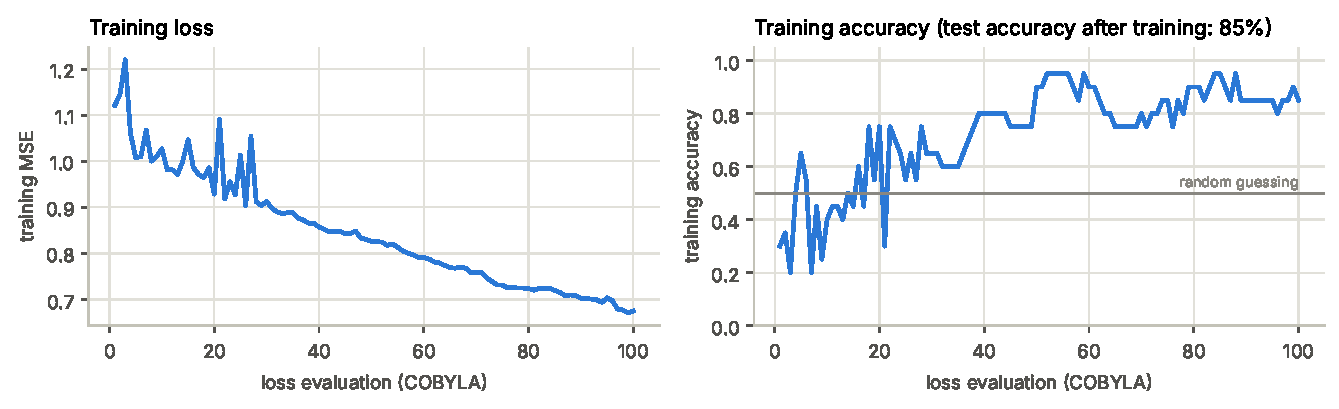
\includegraphics[width=0.86\textwidth]{training_curves}\\
  \small
  \begin{itemize}\itemsep1pt
    \item each point = one COBYLA loss evaluation (20 circuits); the loss falls from \numinitloss{} to \numfinalloss
    \item training accuracy jumps between neighbouring values because 20 images give steps of 5\,\%
    \item the loss is still falling at the end: the 100-evaluation budget, not convergence, stops training
  \end{itemize}
\end{frame}

\begin{frame}[label=fOut]{What the trained QCNN outputs}
  \begin{columns}[T]
    \begin{column}{0.56\textwidth}
      \centering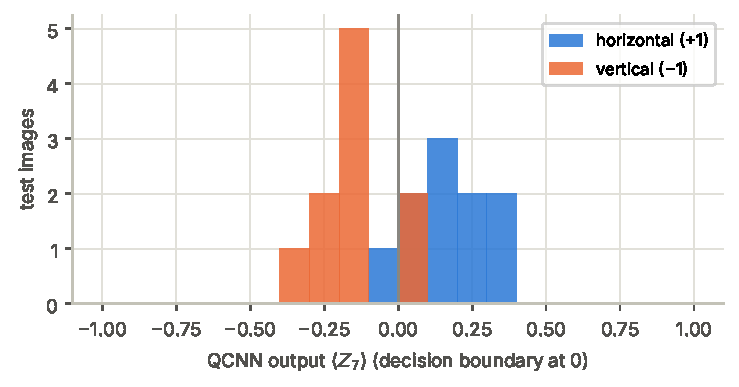
\includegraphics[width=\textwidth]{test_histogram}
    \end{column}
    \begin{column}{0.40\textwidth}
      \small
      \begin{itemize}\itemsep1pt
        \item horizontal images mostly give $\langle Z_7\rangle > 0$, vertical ones $< 0$
        \item but all outputs lie close to 0 (mean $|\langle Z_7\rangle| = \numtestmargin$): low confidence
        \item test: TP \numtesttp, FN \numtestfn, FP \numtestfp, TN \numtesttn; $F_1 = \numtestfone$
        \item test MSE \numtestloss{} vs.\ training MSE \numfinalloss
      \end{itemize}
    \end{column}
  \end{columns}
\end{frame}

\begin{frame}[label=fScale]{Performance benchmarking and scalability \tagillus}
  \begin{columns}[T]
    \begin{column}{0.56\textwidth}
      \centering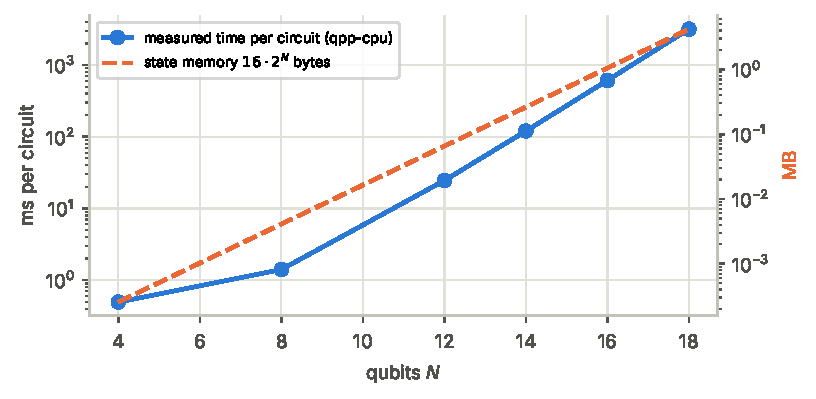
\includegraphics[width=\textwidth]{scaling}
    \end{column}
    \begin{column}{0.40\textwidth}
      \small
      Time of one QCNN circuit (\texttt{cudaq.observe}, \texttt{qpp-cpu}, median of 3) vs.\ qubits.
      \begin{itemize}\itemsep1pt\scriptsize
        \item 18 qubits: \numtimeeighteen{} ms per circuit
        \item training cost $\approx$ evaluations $\times$ images $\times$ time per circuit
        \item README (recorded): 15 qubits, $\approx0.35$ s per circuit, $60 \times 16$ circuits $\approx 5.6$ min, accuracy only 69\,\%
        \item GPU simulation should be much faster (not measured here)
      \end{itemize}
    \end{column}
  \end{columns}
\end{frame}

\begin{frame}[label=fScaleCh]{Scalability challenges}
  \begin{columns}[T]
    \begin{column}{0.5\textwidth}
      \small
      \begin{block}{Simulation}
        \scriptsize memory $16\cdot2^N$; time $\propto$ gates $\times\,2^N$; 30+ qubits need GPUs, 34+ need multiple GPUs or tensor networks.
      \end{block}
      \begin{block}{Training}
        \scriptsize circuits per epoch $= M\times$(evaluations or shift terms); exact gradients cost $\approx 2\times$(gate occurrences) circuits per image;
        optimizer steps grow with the number of parameters.
      \end{block}
    \end{column}
    \begin{column}{0.46\textwidth}
      \begin{block}{Hardware}
        \scriptsize shots ($\sim 1/\epsilon^2$), noise (margins shrink), limited connectivity (SWAPs), queue time; data loading per image.
      \end{block}
      \begin{block}{Trainability}
        \scriptsize barren plateaus, local minima, kernel concentration --- all worsen with size.
      \end{block}
    \end{column}
  \end{columns}
\end{frame}

\begin{frame}[label=fAdv]{Quantum advantage --- and its limits}
  \begin{columns}[T]
    \begin{column}{0.52\textwidth}
      \small
      \key{What is known}
      \begin{itemize}\itemsep1pt\scriptsize
        \item provable separations exist for artificial problems (e.g.\ learning based on discrete logarithms, Liu et al.\ 2021) and for learning from
          \emph{quantum} data (Huang et al.\ 2022)
        \item many claimed exponential speed-ups assume QRAM and low rank; dequantization removes several of them
        \item no demonstrated practical advantage for classical data such as images
      \end{itemize}
      \key{How to test a claim}
      \begin{itemize}\itemsep1pt\scriptsize
        \item strong classical baselines, same data, same budget
        \item large test sets, error bars, several seeds
        \item count all costs: encoding, shots, optimizer steps
      \end{itemize}
    \end{column}
    \begin{column}{0.44\textwidth}
      \begin{alertblock}{This repository}
        \scriptsize The QCNN is simulated on a CPU in seconds; classical methods (rule, kernel SVM) do better on the same task. \texttt{QML.ipynb} makes
        \emph{no} advantage claim, and neither do these slides.
      \end{alertblock}
    \end{column}
  \end{columns}
\end{frame}

\begin{frame}[label=fFuture]{Future research directions}
  \begin{columns}[T]
    \begin{column}{0.5\textwidth}
      \small
      \begin{itemize}\itemsep2pt
        \item learning from \key{quantum data} (sensors, simulations, phases of matter)
        \item \key{geometric / equivariant} QML: architectures that respect the symmetries of the data
        \item trainability without classical simulability: where is the useful middle ground?
        \item \key{error mitigation} and fault-tolerant QML
        \item better \key{data loading} and kernel design avoiding concentration
      \end{itemize}
    \end{column}
    \begin{column}{0.46\textwidth}
      \begin{block}{Natural extensions of \texttt{QML.ipynb}}
        \scriptsize
        \begin{itemize}\itemsep1pt
          \item GPU / \texttt{mqpu} runs at 15--20 qubits
          \item gradient-based training with per-occurrence shift rules
          \item shot-based and noisy training
          \item larger test sets; precision/recall/F1 in the report
          \item classical baselines inside the notebook
        \end{itemize}
      \end{block}
    \end{column}
  \end{columns}
\end{frame}

\begin{frame}{Try it yourself: \texttt{QML.ipynb}}
  \begin{columns}[T]
    \begin{column}{0.5\textwidth}
      \small
      Edit only Section 3:
      \begin{itemize}\itemsep1pt\scriptsize
        \item \texttt{NOISE\_LEVEL = 0.5}: harder task; watch the test accuracy
        \item \texttt{MAX\_ITERATIONS = 300}: does the loss keep falling?
        \item \texttt{IMAGE\_ROWS, IMAGE\_COLS, LINE\_LENGTH = 3, 5, 3} with \texttt{TARGET = "nvidia"} on a GPU
        \item \texttt{OPTIMIZER = "Nelder-Mead"}: compare the curves
        \item different \texttt{SEED}s: how much does the test accuracy vary?
      \end{itemize}
    \end{column}
    \begin{column}{0.46\textwidth}
      \small Reproduce these slides:
      \begin{itemize}\itemsep1pt\scriptsize
        \item \texttt{cd presentations/qml\_source}
        \item \texttt{python make\_figures.py} (re-executes the notebook pipeline and all experiments)
        \item \texttt{latexmk -pdf qml\_lecture.tex}
      \end{itemize}
      Test yourself: \texttt{assessments/QML\_Question\_Paper.pdf} (80 questions) and the separate Answer Book.
    \end{column}
  \end{columns}
\end{frame}

% =====================================================================================
\section{Practice and summary}
\begin{frame}{Exercises}
  \begin{enumerate}\small
    \item Angle-encode the pixel $x = \frac23$ with $R_Y(\pi x)$. Find $P(1)$ and $\langle Z\rangle$.
    \item Amplitude-encode $(3, 0, 4, 0)$. How many qubits? Probability that qubit 1 is 1?
    \item Compute the notebook's kernel $k(\bx, \bx')$ for $\bx = (0, 1, 0.5)$, $\bx' = (0, 0.5, 0.5)$.
    \item $f(\theta + \frac\pi2) = 0.1$, $f(\theta - \frac\pi2) = 0.7$ for a single $R_Y(\theta)$. Find $f'(\theta)$.
    \item How many layers and parameters has the notebook's QCNN for $N = 12$? How many gates?
    \item A swap test gives $P(0) = 0.75$. What is $|\braket{\psi|\phi}|^2$?
    \item How many circuits does one exact gradient of the 8-qubit QCNN loss over 20 images need?
    \item A classifier is right on 45 of 50 test images. Give the accuracy with its standard error.
  \end{enumerate}
\end{frame}

\begin{frame}{Answers}
  \small
  \begin{enumerate}
    \item Half-angle $\frac\pi3$: $P(1) = \sin^2\frac\pi3 = \frac34$, $\langle Z\rangle = \cos\frac{2\pi}3 = -\frac12$.
    \item Norm 5; $0.6\ket{00} + 0.8\ket{10}$; 2 qubits; qubit 1 is always 0: probability 0.
    \item $\cos^2 0\cdot\cos^2\frac\pi4\cdot\cos^20 = \frac12$.
    \item $\frac12(0.1 - 0.7) = -0.3$.
    \item $12 \to 6 \to 3 \to 2 \to 1$: 4 layers, 16 parameters. Conv blocks $(6 + 5) + (3 + 2) + (1 + 1) + 1 = 19$, pool $6 + 3 + 1 + 1 = 11$: $12 + 57 + 44 = 113$ gates.
    \item $2(0.75) - 1 = 0.5$.
    \item $(4\cdot11 + 8\cdot7)\times20 = 2000$.
    \item $0.90 \pm \sqrt{0.9\cdot0.1/50} = 0.90 \pm 0.042$.
  \end{enumerate}
\end{frame}

\begin{frame}{Summary}
  \begin{columns}[T]
    \begin{column}{0.56\textwidth}
      \footnotesize
      \begin{itemize}\itemsep1pt
        \item ML = data + model + loss + optimizer; judge models on independent test data with error bars and baselines.
        \item QML models = encoding + parameterized circuit + measured expectation value, trained in a hybrid loop.
        \item Encodings trade qubits for depth; the fidelity kernel of a product encoding is classically trivial.
        \item Parameter shift gives exact gradients for Pauli rotations; shared or controlled parameters need care.
        \item Trainability (barren plateaus), noise, shots and data loading limit QML.
        \item \texttt{QML.ipynb}: 8-qubit QCNN, 12 parameters, 69 gates, \numtrainacc\,\% / \numtestacc\,\% --- reproduced exactly; simple classical
          methods do better; no advantage claimed.
      \end{itemize}
    \end{column}
    \begin{column}{0.40\textwidth}
      \begin{block}{Further reading}
        \scriptsize
        \begin{itemize}\itemsep0pt
          \item M.\ Schuld, F.\ Petruccione, \emph{Machine Learning with Quantum Computers} (2021)
          \item J.\ Biamonte et al., \emph{Quantum machine learning}, Nature 549 (2017)
          \item I.\ Cong, S.\ Choi, M.\ Lukin, \emph{Quantum convolutional neural networks}, Nat.\ Phys.\ 15 (2019)
          \item M.\ Cerezo et al., \emph{Variational quantum algorithms}, Nat.\ Rev.\ Phys.\ 3 (2021)
          \item NVIDIA CUDA-Q documentation
          \item This repository: \texttt{QML.ipynb}, \texttt{assessments/QML\_*.pdf}
        \end{itemize}
      \end{block}
    \end{column}
  \end{columns}
\end{frame}

% =====================================================================================
\section{Syllabus map}
\begin{frame}{Syllabus coverage: topics 1--32}
  \tiny
  \begin{columns}[T]
    \begin{column}{0.49\textwidth}
\begin{tabular}{rlr}\toprule \# & topic & slides\\ \midrule
1 & Introduction to machine learning & \pageref{fML} \\
2 & Supervised learning & \pageref{fKinds} \\
3 & Unsupervised learning & \pageref{fKinds} \\
4 & Classification and regression & \pageref{fKinds} \\
5 & Training and testing datasets & \pageref{fSplit} \\
6 & Feature engineering & \pageref{fFeat} \\
7 & Loss functions & \pageref{fLoss} \\
8 & Gradient descent & \pageref{fGD} \\
9 & Neural networks & \pageref{fNN}, \pageref{fBackprop} \\
10 & Overfitting and underfitting & \pageref{fFit} \\
11 & Model evaluation & \pageref{fEval}, \pageref{fUnc} \\
12 & Classical ML versus QML & \pageref{fCvQ} \\
13 & Qubits and quantum states & \pageref{fQubit} \\
14 & Superposition and entanglement & \pageref{fQubit}, \pageref{fEnt} \\
15 & Quantum gates & \pageref{fGates} \\
16 & Quantum circuits & \pageref{fCirc} \\
\bottomrule\end{tabular}
    \end{column}
    \begin{column}{0.49\textwidth}
\begin{tabular}{rlr}\toprule \# & topic & slides\\ \midrule
17 & Measurement & \pageref{fQubit}, \pageref{fCirc} \\
18 & Parameterized quantum circuits & \pageref{fPQC} \\
19 & Bloch sphere & \pageref{fBloch} \\
20 & Tensor products & \pageref{fTensor} \\
21 & Unitary operations & \pageref{fGates} \\
22 & Quantum state preparation & \pageref{fPrep} \\
23 & Introduction to QML & \pageref{fQML} \\
24 & Quantum data and classical data & \pageref{fQML}, \pageref{fQData} \\
25 & Classical-to-quantum data encoding & \pageref{fEnc} \\
26 & Basis encoding & \pageref{fBasisAmp} \\
27 & Amplitude encoding & \pageref{fBasisAmp} \\
28 & Angle encoding & \pageref{fAngle} \\
29 & Quantum feature maps & \pageref{fFMap} \\
30 & Variational quantum circuits & \pageref{fAnsatz} \\
31 & Quantum neural networks & \pageref{fQNN} \\
32 & Parameter optimization & \pageref{fOpt} \\
\bottomrule\end{tabular}
    \end{column}
  \end{columns}
\end{frame}

\begin{frame}{Syllabus coverage: topics 33--64}
  \tiny
  \begin{columns}[T]
    \begin{column}{0.49\textwidth}
\begin{tabular}{rlr}\toprule \# & topic & slides\\ \midrule
33 & Hybrid quantum-classical learning & \pageref{fHybrid} \\
34 & Loss functions and gradients & \pageref{fLossOut}, \pageref{fPSC} \\
35 & Parameter-shift rule & \pageref{fPSD}, \pageref{fPSC}, \pageref{fPSF} \\
36 & Measurement and expectation values & \pageref{fCirc}, \pageref{fLossOut} \\
37 & Variational Quantum Classifier & \pageref{fVQC} \\
38 & Quantum Support Vector Machine & \pageref{fQSVM}, \pageref{fKSVM} \\
39 & Quantum kernel methods & \pageref{fKern}, \pageref{fQSVM}, \pageref{fKSVM} \\
40 & Quantum neural networks & \pageref{fQNN}, \pageref{fQCNN} \\
41 & Quantum convolutional neural networks & \pageref{fQCNN}, \pageref{fBlocks}, \pageref{fSize} \\
42 & Quantum GANs & \pageref{fGAN} \\
43 & Quantum PCA & \pageref{fPCA} \\
44 & Quantum clustering & \pageref{fClusRL} \\
45 & Quantum reinforcement learning & \pageref{fClusRL} \\
46 & Quantum data classification & \pageref{fQData} \\
47 & Hybrid quantum-classical architectures & \pageref{fHArch} \\
48 & Barren plateaus & \pageref{fBP}, \pageref{fBPm} \\
\bottomrule\end{tabular}
    \end{column}
    \begin{column}{0.49\textwidth}
\begin{tabular}{rlr}\toprule \# & topic & slides\\ \midrule
49 & Gradient vanishing & \pageref{fBP}, \pageref{fBPm} \\
50 & Expressibility and entanglement & \pageref{fExpr} \\
51 & Circuit depth and trainability & \pageref{fExpr} \\
52 & Noise in QML & \pageref{fNoise}, \pageref{fShots} \\
53 & Quantum model evaluation & \pageref{fEval}, \pageref{fBase}, \pageref{fOut} \\
54 & Classical baseline comparison & \pageref{fBase} \\
55 & Dataset preprocessing & \pageref{fData} \\
56 & Training and testing pipeline & \pageref{fData}, \pageref{fTrain} \\
57 & CUDA-Q implementation & \pageref{fStruct}, \pageref{fLayout}, \pageref{fKernel}, \pageref{fTrain}, \pageref{fGlance} \\
58 & GPU-accelerated simulation & \pageref{fTargets} \\
59 & Multi-GPU execution & \pageref{fTargets} \\
60 & Performance benchmarking & \pageref{fScale}, \pageref{fRec} \\
61 & Accuracy and loss visualization & \pageref{fCurves}, \pageref{fOut} \\
62 & Scalability challenges & \pageref{fScaleCh} \\
63 & Quantum advantage and its limitations & \pageref{fAdv} \\
64 & Future research directions & \pageref{fFuture} \\
\bottomrule\end{tabular}
    \end{column}
  \end{columns}
\end{frame}

\end{document}
